%`
%Read /home/ocean/Documents/PTNR/CulhamFusion/AllPapers/ANNunfolding/BonnerSphere/ThreeAIUnfolding.pdf
%\nonstopmode
\hbadness=100000
\documentclass[a4paper, 12pt]{article}
\usepackage{amsmath,amsfonts,changepage,caption,float,geometry,graphicx,mathtools,pythonhighlight,textcomp,url,verbatim,subcaption,tabularx, longtable} %,parskip
% \usepackage[justification=centering]{subfig}
\geometry{ a4paper, total={170mm,257mm}, left=20mm, top=20mm}

\newcommand{\matr}[1]{\underline{\underline{\textbf{#1}}}}
\newcommand{\ve}[1]{\boldsymbol{#1}}
\newcommand{\pythoncode}[2]{
\begin{adjustwidth}{-1.3cm}{-1.3cm}
\texttt{#1}
\inputpython{#2}{1}{1500}
\end{adjustwidth}
}
\newcommand{\fluenceandactivities}[1]{
\includegraphics[width=11cm]{#1fluence.png}
\includegraphics[width=5cm]{#1activities.png}
}
\usepackage[toc, page]{appendix}
% \usepackage[dvipsnames]{xcolor}
% \definecolor{subr}{rgb}{0.8, 0.33, 0.0}
% \definecolor{func}{rgb}{0.76, 0.6, 0.42}

\begin{document}

\centering


\includegraphics[width=8cm]{CoverPage/UoBlogo.pdf}
\hrule
\bigbreak
\textbf{F}usion Neutron \textbf{Acti}vation Spectra \textbf{U}nfolding by \textbf{N}eural \textbf{N}etworks \\
(FACTIUNN)                                      \\
\hrule
\bigbreak
\begin{minipage}[b]{0.4\textwidth}
    
\includegraphics[height=2cm]{CoverPage/CCFElogo.jpeg}
  \end{minipage}
  \hfill
  \begin{minipage}[b]{0.4\textwidth}
    
\includegraphics[height=3cm]{CoverPage/UKAEAlogo.jpeg}
\end{minipage}
    
\begin{table}[!h]
\centering
\begin{tabular}{rl}
author:&Ocean Wong          \\
       &(Hoi Yeung Wong)    \\
supervisor:&Ross Worrall    \\
Submitted in fulfilment of the requirement for:& MSc. Physics and Technology of Nuclear Reactors \\
date:  &June-September 2019 \\
student ID:& 1625143        \\
\end{tabular}
\end{table}
\hrule
\bigbreak
I warrant that the content of this dissertation is the direct result of my own work and that any use made in it of published or unpublished materials is fully and correctly referenced.

\abstract
Include these things:
\begin{itemize}
    \item Attempted this
    \item Got this result
    \item advice for the future
\end{itemize}
\emph{Keywords:} activation, neutronics, fusion
% \hline
% \twocolumn
\pagebreak
\tableofcontents
\listoffigures
\pagebreak


\chapter{}
\section{Introduction}
%multicols %for two columns % switch by column break.
% \begin{align}
% 	q=\left[\cos(\frac{\theta}{2}),
% 			x\sin(\frac{\theta}{2}),
% 			y\sin(\frac{\theta}{2}),
% 			z\sin(\frac{\theta}{2})
% 			\right]\\
% \intertext{where}
% \begin{pmatrix}
% 	cov(m,m) & cov(m,c)\\
% 	cov(c,m) & cov(c,c)
% \end{pmatrix}
% \end{align}
    
%Bullshit something about the importance of Fusion later in this paper.

In a fusion reactor, the neutron fluence can go up to as high as $1.7 \times 10^{21} cm^{-2}$\cite{14MeVNNeutonYieldCalibration-JET}.
This leads to an unprecedented need of shielding against neutrons of up to 14.1 MeV or higher energies.

Neutrons are notoriously difficult to shield against due to their uncharged nature, and therefore low propensity to interact with matter[citation needed]. To develop effective shielding for various components of the reactor from these high energy neutrons, the energy spectrum of the neutrons created inside the nuclear reactor has to be well understood \cite{TechnologicalExploitationOfDT}.

It is also important to understand the neutron spectrum inside the reactor in order to develop Tritium breeding modules; a Tritium Breeding Ratio TBR$>1$ is essential for making fusion a sustainable source of clean energy \cite{TBMD_Design}.
%Can expand on the Tritium breeding part.
Last but not least, the power output of future fusion power plants can only be quantified when the neutron spectrum is characterised \cite{FusionYieldMeasurementOnJETAndTheirCalibration}.
An accurate measurement of the neutron spectrum is required to properly model the energy distribution of neutrons to be used in neutron transport simulations for the above purposes.
% Additionally, knowing the energy distribution of neutrons is beneficial to advancing the current understanding of the the nuclear processes and scattering interactions inside the reactor [citation needed].

All of the above activities relies on having accurate knowledge of the neutron spectrum. Therefore neutron spectroscopy is a key focus in the diagnostic systems in all fusion reactors.

Incidentally, for the same reason that they are difficult to shield against, neutron energy is also difficult to measure. Neutrons, especially high energy neutrons such as the 14.1 MeV neutrons created in fusion reactors, do not easily deposit their full energy into a sufficiently small detection volume to allow direct measurement\cite{Knoll2010}. Various neutron detectors has been developed to deal with this proble;%Cite any neutron detector, e.g. organic
%Including magnetic proton recoil?
%And fission chambers (energy indep), neutron cameras
however, most of them cannot stand this high neutron fluence at the first wall of fusion reactors without additional shielding that changes the flux profile \cite{ScintillationDetectorResponseFunction}.
The extreme temperature and magnetic fields inside the nuclear fusion reactor compounds the difficulty of employing other means of neutron measurement as most electronics will not be able to function in such environments effectively. \cite{CCDCameraDamage}
%List the other two, but say that neutron activation stands out in the following way:

This is where the technique of activation foil unfolding stands out: By analyzing the level of activations in various elements induced by neutrons, relying on the variation of reaction cross-sections across different elements and energies, one can infer the neutron spectra that was previously present at the first wall.

This is a very robust method as it does not require any active components, thus can be employed for very high neutron fluxes \cite{NSpecHistoricalReviewAndPresentStatus}, as the total number of neutron activation reactions can be controlled by changing the volume of the activation foils used \cite{bethColling_TBMD} according to the anticipated neutron fluence in the next irradiation period, so not to paralyze the $\gamma$ radiation detector. It is also insensitive to $\gamma$ rays, thus removing most of the challenges facing mixed-field spectrometry. \cite{NeutronSpectrometryInMixedFieldsMultiSphereSpectrometers}

The disadvantage of this method is that it has to be time-integrated over the whole irradiation period, thus no information about the temporal variation in the neutron spectrum can be gleamed from its measurements.

Another disadvantage of using neutron activation as the means of measuring the neutron spectrum in a fusion reactor is that it is an indirect method of measurement, requiring the measured reaction rates to be `unfolded' back into reaction rates. This is a `mathematically incorrectly posed ' problem\cite{BirminghamUnfolding}, as will be further explained in the next section (\ref{Neural Network Theory}), requiring an initial guess spectrum to be provided before the unfolding procedure can take place. This is because the number of reaction channels recorded (usually denoted as M) is fewer than the number of neutron groups (usually denoted as N) whose neutron flux we would like to know, i.e. M$<$N, thus this problem is underdetermined (the number of contraints is fewer than the number of variables). The \emph{a priori} has to be used in order to introduce extra information into the problem. However, if this \emph{a priori} spectrum deviates too much from the actual spectrum, then the result of the unfolding will be inaccurate.

To address this problem, an investigation into using neural networks for the purpose of unfolding fusion neutron spectra is presented in this thesis.
Neural networks excels in incorperating previous spectra as \emph{a priori} information, without requiring users to explicitly input an \emph{a priori}.
% It effectively incorperates multiple spectra together as the \emph{a priori}; while MAXED and GRAVEL uses only 1.
Two approaches are proposed. The first one is to use neural networks directly as an unfolding tool; and the second one is to use them as an \emph{a priori} generator, which is then fed into an existing unfolding code, where the actual neutrons spectra is then calculated out of.

\section{Theory}
When a nuclide is placed in the activation module at the irradiation position inside a nuclear fusion reactor (or any other neutron sources), it is activated via one or more nuclear reactions with the incoming neutrons. The probability of interacting with the incoming neutron via reaction $j$ is proportional to the microscopic cross-section $\sigma_j (E)$, where $E$ is the neutron's energy, and reaction $j$ is a neutron-induced reaction, i.e. (n,\textit{any}) reaction.

% The measured activity = (count rate)/(absolute efficiency of set-up at energy for decay of daughter j) /(count period);
% The total number of reaction $j$ = (measured activity)/(probability of daughter's gamma decay per second)

By measuring the activity of reaction $j$'s daughter nuclide in the activation foil (which has a known amount of the initial nuclide) after irradiation, and multiplying it by a correction factor of 
\begin{equation}
    \frac{1}{{1-exp({\lambda_j}T)}}
\end{equation}
the reaction rate $Z_{0j}$ can be obtained. This correction factor accounts for the decay of the daughter nuclide of reaction $j$ which has a half-life of $\lambda_j$, over the period $T$ which is the duration between irradiation and measurement. A more complicated correction factor is required if the irradiation period is comparable to the half-life $\lambda_j$, or if the population of the parent nuclides for reaction $j$ changes over the course of the irradiation. This can be done using FISPACT-II, detailed in \cite{LWP_LTIS}.

The total reaction rate of the $j^{th}$ reaction can then be expressed as a Fredholm integral as follows:
\begin{equation}
    Z_{0j}= \int_{0}^{\infty} R_{j}(E) \phi_0(E) {d}E
\end{equation}
where the reaction rate $Z_{0j}$ has the unit of $s^{-1}$,
%This is a Fredholm equation!! Gotta mention this.
$\phi_0$ is the neutron flux (unit: $cm^{-2} s^{-1} eV^{-1}$), which is a function of energy $E$. The unfolding process aims to find a solution spectrum $\phi$ which approximates the actual spectrum $\phi_0$ as closely as possible. 
%%Note that $\phi$ is commonly used to refer to the neutron fluence in the unfolding context, instead of the neutron flux, as is usually the case in other nuclear physics literature. [citation needed] %cite MAXED and GRAVEL. %i.e. cite the UMG package.

% \textit{Note: In neutron spectra unfolding codes, the quantity that is ultimately of interest to the user is the distribution of neutrons. It doesn't matter whether the unfolded number is a time dependent quantity (neutron flux with unit = $cm^{-2} s^{-1}$) or not (neutron fluence with unit = $cm^{-2}$). Therefore previous papers has made no effort in differentiating one from the other, and simply used $\phi$ for both; sometimes even mixing up the two terms by referring to `flux' as `fluence rate'.} %Can use this paragraph in my PhD.

As for $R$ in the equation above, (which has dimension of area)
\begin{equation}
    R_j(E) =\sigma_{j}(E) \frac{N_A } {A} F_j \rho V
\end{equation}

assuming that there is no self-shielding/down-scattering inside the foil.
$N_A$ is the Advogadro's constant (unit: ${mol}^{-1}$),
$A$ is the molar mass of the parent nuclide for reaction $j$ (unit: g ${mol}^{-1}$),
$F_j$ is reaction $j$'s parent isotope's mass fraction in the foil's constituent material (unit: dimensionless),
$\rho$ is the density of the alloy (unit: g ${barn}^{-1}$ ${cm}^{-1}$),
$V$ is the volume of the foil (unit: ${cm}^3$) Note that $\sigma(E)$ (unit: $barn$)is the only energy dependent component in $R$. %, $\rho$ is the density of the foil; and $V$ is the volume of the foil.

The neutron spectrum can be discretized into N energy bins:
\begin{equation} \label{unfolding equation jth component}
    Z_{0j}= \sum_{i=1}^{N} R_{ji} \phi_{0i}
\end{equation}

where $\phi_{0i}$ is the scalar flux integrated over the energy bin's range 
\begin{equation}
    \phi_{0i} = \int_{E_{i-1}}^{E_i} \phi_{0} d(E)
\end{equation}
, thus having a unit of $cm^{-2} s^{-1}$.

By assuming that the scalar flux distribution inside each energy bin is relatively flat, equation \ref{unfolding equation jth component} calculates $Z_{0j}$ by replacing ($R_j (E), E_{i-1}\le E\le E_{i}$) with 
\begin{equation}
    R_{ji}=R_j (E_{i-1})
\end{equation}

Let there be M neutron-induced reactions whose reaction rate was measured,
\begin{equation}
\begin{split}
    \forall j \in & \{ 1, ..., M \},  \\
    \exists Z_{0j} \in & \mathbb R_{\ge 0}
\end{split}
\end{equation}

Collecting all reaction rates into a vector $\ve{Z_0}$ of $M$-dimensions, one can express eq. \ref{unfolding equation jth component} as a matrix multiplication equation:
    
\begin{equation} \label{unfolding general equation}
\ve{Z_0}=\matr{R} \ve{\phi_0}
\end{equation}

where $\matr{R}$ is a $M\times N$ matrix, termed the \emph{response matrix}. $\ve{\phi_0}$ is an $N$-dimensional vector containing the neutron flux in the each of the $N$ bins. The subscripts 0's denotes that they are the measured/known quantity, as opposed to the conjectured solutions which will appear later in this text.

For nuclear fusion applications, the number of possible reaction investigated $M$ is very limited \cite{MaterialSelection}, as the parent nuclide of each of these reactions must exist in solids which:
\begin{itemize}
    \item can be manufactured into specified shape and thickness, with well measured number density and impurity contents,
    \item are safe to be handled,
    \item has a threshold energy in the region of interest (in the MeV range),
    \item has well-characterised cross-section values in nuclear data libraries (see \cite{MaterialSelectionASTM})
    \item has stable parent isotope and daughter isotopes of medium length half-lives such that it can be activated and measured.
\end{itemize}
in practice, very few types of metals/alloys can be used in these systems. For the ACT in JET in particular, in recent experiments, only 7 types of foil materials and 11 reactions were examined. \cite{LWP_LTIS}

Meanwhile, the number of bins, $N$, can be arbitrarily high. For some investigations, such at the one in \cite{EmbargoPaper_LWP} it goes up to 709 bins. 
This makes the unfolding problem a strongly underdetermined one.

In the mathematical sense of the problem, an inverse does not exist. This is because, theoretically, multiple neutron spectra, say $\ve{\phi_0}$ , $\ve{\phi_1}$ and $\ve{\phi_2}$, can give the same set of reaction rates $\ve{Z_0}$, so there is no correct, unique choice of mapping of $\ve{Z_0}$ back to $\ve{\phi_0}$ , $\ve{\phi_1}$ and $\ve{\phi_2}$. 
% A conceivable situation is detailed below as an example:

% The three spectra $\ve{\phi_0}$, $\ve{\phi_1}$, $\ve{\phi_2}$ has identical flux values in all but the first two energy bins:

% \begin{itemize}
%     \item $\ve{\phi_0}$ has a flux of $0                cm^{-1} s^{-1}$ in the $1^{st}$ bin and a flux of $2 \times 10^{10} cm^{-2} s^{-1}$ in the $2^{nd}$ bin;
%     \item $\ve{\phi_1}$ has a flux of $2 \times 10^{10} cm^{-2} s^{-1}$ in the $1^{st}$ bin and a flux of $1 \times 10^{10} cm^{-2} s^{-1}$ in the $2^{nd}$ bin;
%     \item $\ve{\phi_2}$ has a flux of $4 \times 10^{10} cm^{-2} s^{-1}$ in the $1^{st}$ bin and a flux of $0                cm^{-2} s^{-1}$ in the $2^{nd}$ bin;
% \end{itemize}

% And the reaction cross-sections in this energy range (very low neutron energy/thermal energy) for all but the $1^{st}$ reaction is vanishingly small, as all other reactions than the $1^{st}$ reaction are threshold reactions.

% If the first two columns of the response matrix \matr{R} are given as follows:
% \begin{align}
%     R_{1,j} = \delta_{1j}(5 \times 10^{-11}) cm^2 \\
%     R_{2,j} = \delta_{1j}(1 \times 10^{-10}) cm^2
% \end{align}
% where the $\delta$ used is the Kronecker delta,

% then one can see that $\ve{\phi_{0}}$, $\ve{\phi_{1}}$ and $\ve{\phi_2}$ will all lead to the same reaction rate $Z_{0}$. This is because, in each of these cases, the first two bins of each of the $\ve{\phi}$ contributes the same amount of reaction rate of 2 counts $s^{-1}$ to the $1^{st}$ reaction rate ($Z_{0j}$ where j=1), ultimately resulting in the same measured reaction rate of $\ve{Z_{0}}$.

Such an inverse problem is termed `mathematically incorrectly posed'. \cite{BirminghamUnfolding}

%I'll skip the bit about the additional problem of lack of variations across cross-section profiles leads to high condition number i.e. worse unfolding performance.

\subsection{General unfolding methods} \label{general methods}
The most straight-forward way of getting back a solution $\phi$ is by using the Moore-Penrose inverse matrix. This matrix inversion operation generalizes the usual matrix inversion operation for square matrices, where the $M\times N$ response matrix \matr{R} in equation \ref{unfolding general equation} is inverted into an $N \times M$ matrix $\mathbf{\underline{\underline{R}}^{-1}}$, so that $\phi$ can be obtained by $\ve{\phi} = \mathbf{\underline{\underline{R}}^{-1}} \ve{Z_0}$. However, this method is the equivalent of rotating a 2-D photo of a 3-D object from a horizontal position to an upright/tilted position: the solution is still ``trapped" in a flat, M-dimensional manifold within the N-dimensional solution space.

Therefore to start the unfolding process, extra information has to be given to the program. This is termed the \emph{a priori} spectrum.

The most general unfolding program can, ideally, find a solution $\ve{Z}$, \matr{R} and $\ve{\phi}$ \cite{theorypdf}, such that their overall deviation from the measured reaction rates ($\ve{Z_0}$), expected response matrix ($\underline{\underline{\mathbf{R_0}}}$), and the initial guessed neutron spectrum ($\ve{\phi_0}$), is minimized. The deviation of the solution reaction rates from the measured reaction rate is calculated from its covariance matrix $\underline{\underline{\mathbf{S_Z}}}$, as the $(\chi^2)_Z = Z^T \underline{\underline{\mathbf{S_Z}^{-1}}} Z$. Equivalently the deviation of $\ve{\phi}$ from $\ve{\phi_0}$ and \matr{R} from $\underline{\underline{\mathbf{R_0}}}$ can be calculated from their respective covariance matrix..

\subsection{Current practice}
In practice, there is always uncertainty associated with the cross-section values provided by the nuclear data libraries \cite{fluence_rate_correction_factors}. This is known as the ``ambiguity" of the response matrix. To reduce the complexitiy of the problem, however, the ambiguity in the response matrix is nearly always ignored, by assuming that the response matrix $\underline{\underline{\mathbf{R_0}}}$ is accurately and precisely defined, fixing the response matrix during the solution search. This reduce the number of dimensions in the solution search by $M\times N$, massively reducing the computational complexity. It also assumes that the covariance matrix of the reaction rates is diagonal, i.e. there are no covariance across different reaction rates.

Some programs, such as GRAVEL\cite{ManfredMatzkeHEPRO} and SAND-II\cite{SAND-II}, simply start their iterative solution search from this \emph{a priori} spectrum, with the aim of minimizing the $\chi^2$ (which measures the deviation of $\ve{Z}$ from $\ve{Z_0}$); while others, such as MAXED \cite{MAXED1998Reginatto} add the deviation of the solution spectrum from the \emph{a priori} spectrum ($\ve{\phi}$ from $\ve{\phi_0}$) on top of the deviation of the solution reaction rates from the measured reaction rates ($\ve{Z}$ from $\ve{Z_0}$) when evaluating the $\chi^2$.
%cite MAXED, SAND-II and GRAVEL

%Cite papers on properly selecting an a priori?
Current fusion neutron measurements relies on MCNP simulations heavily to supplement their unfolding procedure. They use MCNP model of thre reactor to calculate a neutron spectrum, which is used as the \emph{a priori} \cite{MatzkeUnfoldingProcedure} \cite{InternalReportOnDeliverables_LWP}; and the response matrix is usually obtained in the same way as well \cite{bethColling_TBMD}.

\subsection{Neural Networks} \label{Neural Network Theory}
Neural networks, on the other hand, learns the relationship between reaction rates and the original neutron spectrum. Ideally it will make use of information in previous neutron spectra, effectively bypassing the problem of underdetermination.

A typical neural network learns the relationship between the inputs (the two nodes in the leftmost layer in Figure~\ref{SimpleNNArchitecture}) and outputs (the node in the rightmost layer in Figure~\ref{SimpleNNArchitecture}) of a function via training, thus becoming an approximator for that function.

\subsubsection{Forward Propagation}
\begin{figure}[H]
    \centering
    \includegraphics[height=5cm]{/home/ocean/Documents/PTNR/CulhamFusion/Presentation2/SimpleNNArchitecture.png}
    \caption{Illustration of the topology of a typical neural network} \label{SimpleNNArchitecture}
\end{figure}

The inputs to the neural network are known as ``features" and the outputs are known as the ``labels".

In the context of neutron spectrum unfolding using neural networks, there are M features (reaction rates $Z_j$ for $1\le j\le M$) and N labels (neutron flux in each bin $\phi_j$ for $1 \le j \le N$). 

The ``activation" $A_i$ of the $i^{th}$ node refers to the value that it takes.
$w_{ij}$ denotes the ``weight" of each connection from the $j^{th}$ node to the $i^{th}$.

When the activations in the input layer ($A_j$) are known, the activation in the next layer (in this case, the first hidden layer) is calculated as follows:
\begin{equation} \label{forwardpropagation}
    A_i = \sigma_i\left({\sum_{j} (w_{ij}A_j) + b_i}\right)
\end{equation}
$b_{i}$ denotes a ``bias" value which will be added onto the sums in front of each node before it is parsed through the activation function $\sigma_i$.
The activation function is usually denoted as $\sigma_{i}$, i.e. it is possible to use different activation functions for different nodes $i$; however the common practice is to use the same type of activation function across the whole layer, or even across all nodes and all layers of the neural network. The typical function chosen is the ReLU function (Figure~\ref{ReLU}), i.e. for all layers, and for all values of $i$, as it is one of the simplest non-linear function whose gradient can be computed quickly.


\begin{equation}
    \sigma_i(x) = ReLU(x) = \frac{|x|+x}{2}
\end{equation}
\begin{figure}
    \centering
    \includegraphics[height=3cm]{/home/ocean/Documents/PTNR/CulhamFusion/Presentation2/ReLU.png}
    \caption{A ReLU function (a rectifying function)}\label{ReLU}
    Abscissa=function's input; ordinate=function's output.
\end{figure}

Equation~\ref{forwardpropagation} is applied recursively to calculate the activations in the immediate next layer. For example, to calculate the activations in second layer (i.e. the output layer) in Figure~\ref{SimpleNNArchitecture} simply by swapping the indices in for the indices of the next layer: $i\mapsto h$, $j\mapsto i$. This process is known as forward propagation.

\subsubsection{Backpropagation}
    The weights $w$ and biases $b$ are known as the \underline{parameters} of the neural network. This is in contrast with the term ``hyperparameters", which are the numbers that describes the topology of the neural network, i.e. number of layers, number of nodes in each layer, learning rate (see section \ref{sec:training} below), etc. During the training phase of the neural network, these parameters are adjusted so that the neural network's predicted output values align with the true output values more closely. This deviation of the predicted label from the true label is termed the ``loss value", and can be calculated in a variety of manner (see Section \ref{unfolding inverse equation} for the loss value metrics considered in this investigation). For the moment let's assume it is calculated as the mean-squared value, i.e. same as the $\chi^2$ value familiar to physicists.

    The process of adjusting parameters to reduce the loss value is known as backpropagation, as the `desired' change to each weight and bias (calculated from the gradient of the loss value with respect to $w$ or $b$, i.e. $\frac{\partial (loss)}{\partial w}$ or $\frac{\partial (loss)}{\partial b}$) is obtained by tracing the change in the output layer back to the weight and biases of each layer.

    For the neural network to converge on a stable set of parameters (i.e. a minimum value of the loss value in the parameter space), features are usually normalized before they are given to the neural network. This reduces the difference in variance across each feature, allowing the neural network to take a more direct path when gradient-descending to the set of parameters that achieves minimum loss value, instead of an oscillatory approach to the minimum loss value\cite{AndrewNgNormalization}, thus reducing the number of steps required to train the neural network.

\subsubsection{Universal approximation theorem}
    Before diving into the details of neural network training, it is beneficial to see how a neural network can approximate any function.

    The key to its ability of approximating functions lies in the non-linear activation function. 

    \begin{figure}[H]
        
    \begin{center}
        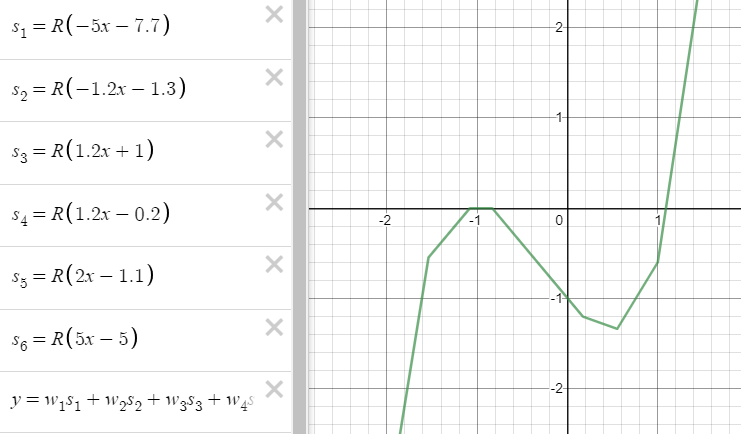
\includegraphics[height=5cm]{PPT/UniversalApproximationTheorem.png}
        \caption{A cubic function approximated by a neural network}\label{UniversalApproximationTheorem}
    \end{center}
    This neural network has 1 hidden layer containing 6 neurons.
    Here, $R$ is the alias for the ReLU function (see Figure~\ref{ReLU}), abscissa is the input layer neuron's activation value (feature); and the ordinate is the output layer neuron's activation value (label), obtained by summing over the product of the activation of the $i^{th}$ neuron (aliased as $s_i$) with the weight of its connection to the final layer (aliased as $w_i$).
    The weights and bias to the first layer is already defined on-screen inside the brackets of the first six lines; while the weights and bias to the second layer (output layer) is defined off screen.
    \end{figure}
    
    Figure~\ref{UniversalApproximationTheorem} is a crude representation of how a 1-hidden-layer neural network can approximate a cubic function. A single hidden layer neural network with one scalar input and one scalar output is able to approximate any non-linear functions, provided that there are enough neurons in the hidden layer.

    The weights $w_i$ scales each ReLU function; whereas the bias to the first layer (defined as the second term inside each of the bracket in the first six lines) changes the horizontal offset of each ReLU function. The bias to the second layer controls the vertical offset of the whole function. Summing them up leads to the output in Figure~\ref{UniversalApproximationTheorem}.

    Even with only six hidden neurons (only 19 parameters), it is able to reasonably approximate a cubic function within the visualized domain. Obviously this approximation to the cubic function can be improved by increasing the number of neurons available in the neural network, provided that there are enough training data to cover the domain densely.

    Armed with this intuition, the notion of a neural network being able to approximate any function becomes conceivable, even if the function has vectorial inputs and outputs. %rewording?

\subsubsection{Training the neural network}\label{sec:training}
    Before adjusting the parameters, a fraction of the data is drawn out and reserved for \underline{testing}. The remaining is used as the \underline{training} dataset. These ``training" and ``testing" data are chosen in such a way that they cover the same range of domain and co-domain in the feature- and label-space respectively.
    
    The parameters are adjusted in iteratively to minimize the loss value. Each step requires calculation of the gradient value over the entire dataset, known as an ``epoch", obtained by calculating the average $\frac{\partial (loss)}{\partial w}$ or $\frac{\partial (loss)}{\partial b}$ over the entire training dataset. The parameters is adjusted according to an algorithm known as the ``optimizer"; this algorithm may require some more hyperparameters, such as the ``momentum", ``acceleration" term to be defined. When further training no longer improves the loss value over the training set (i.e. the ``training loss"), training can be stopped, and the parameters are then fixed at their final values. The size of each step is calculated as (learning rate)$\times$(gradient of the loss value in parameter space)

    The performance of the neural network is then evaluated over the testing set to obtain an average loss value, known as the ``testing loss". If the testing loss is much higher than the training loss, it signifies that the neural network was ``overfitting", i.e. it reached a minimum training loss by ``memorizing" the relationship between training features and training labels, and is unable to generalize these relationships to the testing set. This may suggest that the neural network is too complex, i.e. has too many nodes or neurons.

    Apart from reducing the complexity of the model, various techniques exist to reduces overfitting, including weight-regularization and dropout \cite{TensorflowOverfitting}. Weight regularization ensures that the numerical values of weights $w$ remains small; while dropout effectively removes a specified fraction of the connections at each layer. However, these techniques are not applied.

    However, one of the most widely used method of reducing overfitting is by measuring the validation loss. A small subset of the training data is reserved and not used for backpropagation during the training, but its loss value (known as the ``validation loss") is calculated at each epoch also. This amounts to calculating the loss value of the neural network's prediction on a set of data that it has never seen before as well. When the validation error stops decreasing, then one can be sure that the neural network has stopped identifying general patterns which applies across both the validation set and the training set, and begin memorization. The training can be stopped at this point.

    This method is called ``Early Stopping"; it catches the neural network before it begins overfitting aggressively.

\subsubsection{Applying neural network to the unfolding problem}
    To apply neural networks as unfolding tools, we will want neutron spectra as the output and reaction rates as the input, i.e. M features (reaction rates $Z_j$ for $1\le j\le M$) and N labels (neutron flux in each bin $\phi_j$ for $1 \le j \le N$).

    By using a neural network to do the unfolding, we are assuming that the inverese equation (below) exist,

    \begin{equation} \label{unfolding inverse equation}
        \ve{Z} = \mathbf{\underline{\underline{R}}^{-1}} \ve{\phi}
    \end{equation}
    
    i.e. all reaction rates can be unfolding back to one and only one unique solution spectrum. Ideally, the set of all possible solution for the neutron spectrum $\ve{\phi}$ can be expressed as a linear sum of M or fewer basis vectors due to the contraints of various physical processes. The role of the neural network is to identify these M- bases vectors, and relate them to the M reaction rates.

    Several metrics were considered for the neural networks. Since the neural networks' goal is to predict a set of labels (solution spectrum) $\phi_{pred}$ that is identical to the true spectrum $\phi_{0}$ when given the set of features $Z_{0}$ corresponding to the set of labels $\phi_{0}$, the loss function must have a minimum at $\phi_{pred}=\phi{0}$.

    This loss value is also expected to scale its penalization according to the true flux $\phi_{0}$. Large deviation when $\phi_0$ is large should be penalized by the same amount as with small deviations when $\phi_{0}$ is small. For example, over-predicting the to flux at the 14.1 MeV peak by, say, 10\%, in a DD-operation, should be given the same penalty as over-predicting the 14.1 MeV peak flux in a DT-operation by 10\%, despite the fact that $\phi_{0}(E=14.1 MeV)$ is much smaller for the same TOKAMAK in a DD campaign than in a DT campaign.

    Several of such functions comes to mind; they include:

    \begin{itemize}
        \item cross entropy, $H(\phi_{pred}, \phi_{0}) = \sum_i^N \bigg(\phi_{pred}(E_i)(ln(\phi_{pred}(E_i)) - ln(\phi_{0}(E_i)))\bigg)$ (See \cite{Johnson-Shore-Deriv})
        \item Average distance in $L^P$ log-space $=\bigg(\sum_i^N(log(\phi_{pred})-log(\phi_{0}))^p\bigg)^{\frac{1}{p}}$
        which is a generalization of mean squared error and mean absolute error.
        \item mean fractional deviation, $MFD (\phi_{pred}, \phi_{0}) = \sum_i^N \bigg|\frac{\phi_{pred}(E_i)-\phi_0(E_i)}{\phi_{0}(E_i)}\bigg|$
    \end{itemize}

    In the end, the following functions were chosen as they were the default functions available from tensorflow; using these functions minimizes the room for human error and development time.

    Let there be L features-labels pairs in the datatset. The loss values are defined as:
    \begin{itemize}
        \item mean squared error:
        \begin{equation}\label{MSE}
            MSE(\ve{\phi_{pred}},\ve{\phi_0}) = \frac{1}{L} \sum_{k}^L \sum_i^N \bigg( log_{10}\big(\phi_{pred,k}(E_i)\big)-log_{10}\big(\phi_{0,k}(E_i)\big) \bigg)
        \end{equation}
        \item mean pairwise squared error:
        \begin{equation}\label{MPSE}
            MPSE(\ve{\phi_{pred}}, \ve{\phi_{0}}) = \frac{1}{L} \sum_{k}^L \sum_i^N \sum_q^N \left( log_{10}\left(\frac{\phi_{pred,k}(E_i)}{\phi_{pred,k}(E_q)}\right)-log_{10}\left(\frac{\phi_{0,k}(E_i)}{\phi_{0,k}(E_q)}\right) \right)
        \end{equation}

    \end{itemize}
    The neural networks in this investigation differ from the typical neural network, in that the latter has fewer labels than features output ($N \le M$); and that, since the features is related to the labels via a physical process, the inverse function for turning labels back into features exist (equation~\ref{unfolding general equation}), and is assumed to be deterministic.
    
    This allows for an additional information to be supplied to the neural network during the training stage:
        
    \begin{itemize}
        \item mean squared error including folded reaction rates:
        \begin{equation}\label{MSE_including_folded_reaction_rates}
            MSE_{\text{including\_folded\_reaction\_rates}}=MSE(\ve{\phi_{pred}'},\ve{\phi_{0}'})
        \end{equation}
        \item mean pairwise squared error including folded reaction rates:
        \begin{equation}\label{MPSE_including_folded_reaction_rates}
            MPSE_{\text{including\_folded\_reaction\_rates}} = MPSE(\ve{\phi_{pred}'},\ve{\phi_{0}'})
        \end{equation}
        % \item loss function: pairwise, tried using cosine distance but it didn't work because it simply gave NaN's.
    \end{itemize}
    Where $\ve{\phi'}$ is the $\ve{\phi}$ and $\ve{Z}$ vector concatenated together,
    \begin{equation}\label{NNregularization}
        \ve{\phi'} = [\phi_1, ..., \phi_N, Z_1, ..., Z_M]
    \end{equation}
    and Z is, in turn, obtained by equation \ref{unfolding general equation}:

    \begin{align}\label{unfolding general equation prediction}
        \ve{Z_{pred}} &= \matr{R} \ve{\phi_{pred} }\\
        \ve{Z_{0}} &= \matr{R} \ve{\phi_{0} }
    \end{align}

    This is analogous to the technique of regularization\cite{FisherRegularization} in normal unfolding procedures, where both deviation from the \emph{a priori} spectrum and the reaction rates are calculated and used as the $\chi^2$ value. In this case, the regularization constnat (weight of the neutron flux's deviation relative to the reaction rates' deviation) is simply chosen as 1.

    These two metrics will give loss value = 0 when $\phi_{pred}$ and $\phi_0$ matches perfectly; but the neural network will be penalized by an additional amount if it makes a mistakes in the spectrum that leads to a greater deviation of the $Z_{pred}$ from the $Z_{0}$ (which is a mistake that other linear/non-linear least-square unfolding codes such as MAXED and GRAVEL will not make. This effectively incorperate some physics into the neural network with the hopes of improving its accuracy.

\section{Literature review}\label{Literature review}
There are no previous attempts of unfolding fusion neutron spectra using neural networks. Therefore this technique is entreily new and not applied.

Some work has been carried out in the field of neutron spectrum unfolding using neural networks. Only one of them are directly related to the method of activation foil neutron spectrum unfolding \cite{Accelerator-basedANNUnfolding}, which has a more pathological response matrix than the other two methods typically discussed in unfolding (Bonner Spheres and liquid scintillators). The condition number of the response matrix (i.e. the ratio of the maximum to minimum singular value\cite{MATLAB}) is likely worse due to the similarities between reaction cross-sections as dictated by nuclear physics; unlike in the other two detectors, where the response matrix is almost guaranteed to be lower-triangular matrix, where the response of each Bonner sphere/ scintillation pulse height is guaranteed to be linearly independent from each other, so that the condition number is to be small, i.e. they are less ill-conditioned than the problem of activation foil neutron spectrum unfolding. Therefore unfolding these two types of spectra are not as difficult as unfolding neutron spectra from activation foil.

For the purpose of neutron spectrum measurement in a nuclear fusion reactor, which has very high neutron and $\gamma$ fluence compared to fluences typically found in medical physics and in fission reactors where Bonner spheres and liquid scintillator neutron measurement and unfolding are used. These two methods are unsuitable for measuring fusion neutron energies directly due to their low radiation tolerance relative to the method of activation foil. However, this does not mean the work of neural network unfolding of neutron spectrum from Bonner Spheres measurements
\cite{Rodrigues-UnfoldingCompuerCodeBasedOnANN} %7:10:75 & a momentum =0.1 and a learning rate= 0.1, mse = 1e−4 and a trainscg learning function
\cite{RDANNM} %7:14:31
\cite{ANNDoseQuantitiesPrediction} %Fully determined: 6:16:10:6
\cite{ClaudiaC.BonnerSphereNNUnfolding} % 10:50:52 (not as underdetermined)
and liquid scintillator measurements
\cite{ANN-ModifiedLeastSquare} %Not even under-determined; simply being lazy. (Square)
are not useful for fusion neutron spectra unfolding. They provide useful references of neural network topologies useful for neutron spectrum unfolding (Table~\ref{NNtopology}).

\begin{table}
\begin{tabularx}{\textwidth}{cXX}
Source & topology of NN & comment \\
\hline
\cite{Rodrigues-UnfoldingCompuerCodeBasedOnANN} & 7:10:75 & optimum: momentum =0.1, learning rate= 0.1, activation function = trainscg\\
\cite{RDANNM} & 7:14:31 & optimum: learning rate= 0.1, optimal momentum = 0.1, activation function = trainscg (same author as \cite{Rodrigues-UnfoldingCompuerCodeBasedOnANN})\\
\cite{ANNDoseQuantitiesPrediction} & 6:10:16:6 & Fully determined system \\
\cite{ANN-ModifiedLeastSquare} & 1 input layer : 2 hidden layer : 1 output layer & Fully determined system \\
\cite{LancasterNN} & 50:50:1 & over-determined (for fluence estimation)\\
\cite{ClaudiaC.BonnerSphereNNUnfolding} & 10: 50: 52 & used for unfolding monoenergetic and continuous spectra\\
\end{tabularx}
\caption{Topology of all of the feed-forward neural networks used for neutron spectra unfolding found in literature.}\label{NNtopology}
\end{table}

They also offer some insight as to how to overcome data the challenge of data scarcity. Namely, with Radial Basis Function Neural Networks (RBFNN) and General Regression Networks (GRNN), which are subsets of Probabilistic Neural Networks (PNN). They are more intricately designed than the typical Feedforward Neural Network (FNN), which is the type of neural network that has been discussed in this thesis so far.
But neutron spectra unfolding with RBFNN\cite{RBF-NN}\cite{ThreeAIUnfolding} and GRNN\cite{NNNeutronFluenceAmbientDoseEquivalent}\cite{unfoldingCodeBasedOnGeneralizedRegressionANN}\cite{ThreeAIUnfolding} are more complicated than unfolding, so in thesis only FNN will be investigated in details; further investigation into using RBFNN and GRNN may follow from this thesis, in an attempt to improve fusion neutron spectrum unfolding performance.

In addition to having a more under-determined matrix than all of the cases displyed in Table~\ref{NNtopology} (number of input nodes = 11; number of output nodes = 175), the problem of unfolding fusion neutron spectra comes with the lack of data:
There are very few existing nuclear fusion facilities in the world, many of which do not have a first-wall similar to JET, ITER or DEMO, where tritium is expected to be bred, and neutron spectra measurement is paramount. Since the first wall condition will affect the plasma physics and the neutron scattering greatly, very few existing fusion neutron spectra are useful for training the neural network. They mainly consist of measurements from JET and modelling results from ITER. (This will be discussed further in Section~\ref{RealResults}.)

Some of these authors\cite{ThreeAIUnfolding} have also attempted to unfold neutron spectra via other artificial intelligence methods, such as Genetic Algorithm (GA). There are some interest on this topic\cite{SVitishaGeneticAlgorithm}\cite{HighResGeneticAlgorithm}, but recent work here in CCFE has shown that GA is unpromising for the purpose of unfolding fusion neutron spectra \cite{R.WorrallThesis}. For completeness, other AI methods that were considered for the purpose of neutron spectra unfolding includes Particle Swamp \cite{ParticleSwamp_NE-213} and Artificial Bee Colony \cite{BeeColony}. None of these methods will be considered in detail as it is beyond the scope of this thesis.

\section{Proof of concept on simulated spectra}
To demonstrate that the neural network is able to unfold neutron spectra at all, simple synthetic neutron spectra were created and folded through a response function, and neural networks were used to unfold them. These synthetic neutron spectra are simple in the sense that there are no physical processes modelled/considered while creating them, thus cannot be used to represent real world data.

\subsection{Fully determined case}
A square response matrix consisting of $5\times5$ randomly picked numbers (uniformly distributed across $1\le R_{ji}\le50$) was generated.

A set of 100 spectra, each containing 5 randomly picked numbers (uniformly distributed across the range $1\le\phi_i\le15$) were also generated. They are regarded as the ``true" neutron flux distributions. The ``true" reaction rates corresponding to each spectrum was obtained by folding it through the response matrix according to equation \ref{unfolding general equation}. These form the features and labels respectively.

A single neural network with 0-hidden layer was able to predict the remaining labels (i.e. labels in the testing set) from the features perfectly after 10000 epochs of training over half the dataset (i.e. the training set consist of the first 50 features-labels pair). Note that at this stage, the neural network has not logarithmized the features' or the labels' numerical values in its pre-processing step, i.e. its loss function calculates the deviation in linear-space instead of log-space in equation \ref{MSE}, and regressing on the original value of the features, instead of $log(\text{features})$. This was done since the features are uniformly distributed within the same magnitude, so feature normalization is not needed.

The perfect replication of the results is an expected and trivial result, as a 0-hidden-layer neural network is merely a matrix multiplication equation. Further examination of the weights (by enabling eager\_execution\_mode in tensorflow before re-training the neural network) shows that the weights connecting the input to the output layer forms a matrix that is identical to the transpose of the inverse matrix $\mathbf{\underline{\underline{R}}^{-1}}$ up to 3 significant figure. The difference after the $3^{rd}$ (or more) significant figure were attributed to rounding errors, and the fact that the learning rate (i.e. Adam Optimizer's default learning rate of 0.001) was too big for the neural network to settle into the minimum in the parameter space properly.

The idea of logarithmizing the numerical values of features and labels in the pre-processing step were then introduced and tested on this dataset.

Since logarithms destroys the linearity of this problem, two hidden layers were added to account for the increased complexity of the problem. (Preliminary experimentation showed that adding only one hidden layer is insufficient, as the loss value does not go down as far as with the two hidden layer neural network.)

The neural network was still able to reproduce the original spectra with a somewhat satisfactory level of accuracy after training for 10000 epoch at a learning rate=0.001 over the 50 training data. Training was done using the Adam algorithm, which is the default tensoflow algorithm. Figure~\ref{5x5} contains 4 example plots from the testing set, as predicted by the neural network.

\begin{figure}
\centering
\includegraphics[height=3cm]{/home/ocean/Documents/PTNR/CulhamFusion/Presentation2/FewChannels_fullydetermined/13simple_log.png}
\includegraphics[height=3cm]{/home/ocean/Documents/PTNR/CulhamFusion/Presentation2/FewChannels_fullydetermined/14simple_log.png}\\
\includegraphics[height=3cm]{/home/ocean/Documents/PTNR/CulhamFusion/Presentation2/FewChannels_fullydetermined/15simple_log.png}
\includegraphics[height=3cm]{/home/ocean/Documents/PTNR/CulhamFusion/Presentation2/FewChannels_fullydetermined/16simple_log.png}
\caption{The spectra predicted by a 2-hidden-layers neural network (with 16 nodes per layer) on a fully determined system.} \label{5x5}
Abscissa: neutron bin number; ordinate: neutron flux (arb. units)\\
The loss function used is as defined in equation~\ref{MSE}.
% Edit graph to give x-y axes labels.
% See /home/ocean/Documents/GitHubDir/unfolding/unfolding/unfoldingsuite/neuralnetwork/simplecase/log_simple_2_layer_error_variation.png for training progress graph
\end{figure}
% list of all spectra plotted together /home/ocean/Documents/GitHubDir/unfolding/AllSpec.png

As expected, larger deviations were observed when the absolute value of $\phi_{0i}$ is high, as the loss value contribution from each $\phi_{pred\:i}$ is proportional to $\frac{log_{10}(\phi_{0i})}{log_{10}(\phi_{pred\:i})}$

\subsection{Underdetermined case}\label{Underdetermined case}
% Creating simulated spectra by data augmentation
To demonstrate that the neural network is capable of performing the unfolding procedure in an underdetermined condition, 2100 spectra were made from 7 fusion neutron spectra, and then used to train and test the neural network. The 7 spectra used are listed in Table~\ref{DataAugmentationSource}.

\begin{table}
\begin{tabularx}{\textwidth}{ccX}
Code & reactor\\
\hline
JAEA-FNS & JAEA Fusion Neutron Source D-T\\
Frascati-NG & ENEA Frascati Neutron Generator D-T\\
ITER-DD & Magnetic confinement fusion, ITER D-D\\
ITER-DT & Magnetic confinement fusion, ITER D-T\\
DEMO-HCPB-FW & DEMO fusion concept He-cooled pebble bed, first wall\\
JET-FW & Joint European Torus, first wall vacuum vessel\\
NIF-ignition & Inertial confinement fusion, NIF ignited\\
\end{tabularx}
\caption{The neutron spectra used as the starting point for creating more simulated fusion neutron spectra, obtained from \cite{FISPACT_reference_spectra} }\label{DataAugmentationSource}
\end{table}
The data were rebinned into a modified Vitamin-J group structure, where the last 4 (highest energy) bins are discarded to avoid the need of extrapolating some of the spectra beyond their recorded energy ranges.

Each neutron spectrum was parametrised as a sum of 3-7 normal and log-normal distributions(see Figure~\ref{Parametrisation}). The full table of the parameters used to parametrise the spectra is listed in Table~\ref{ParametrisationParameters}. The parametrisation was carried out using a parameterised code currently under development at CCFE.

Each simulated new spectrum is created using the following procedure: using the parametrised representation of one of the above spectra, 40\% of these distributions in the parametrised representation were randomly selected to have their amplitudes of scaled up/down by a random factor(picked from a lognormal distribution with $\mu =0, \sigma = 1$), leaving the remaining 60\% of them un-perturbed.

This process was repeated 300 times for each spectrum in Table~\ref{DataAugmentationSource}, giving the 2100 spectra in Figure~\ref{SimulatedCollection}.

% Further increase in complexities (number of layers and numebr of nodes per layers) yield no significant improvement in the fit. This is because increasing the complexity further will simply lead to over-fitting, as the neural network `memorizes' the relationship between features and labels. This was reflected by the continual decrease in the loss value over the training dataset, while the loss value over the validation dataset stops improving.
\begin{figure}
\centering
    \begin{subfigure}[b]{.4\linewidth}
        \includegraphics[width=\linewidth]{/home/ocean/Documents/GitHubDir/unfolding/unfolding/unfoldingsuite/neuralnetwork/demogenerator/7_NIF_Ignition.png}
        \caption{An example of parametrisation performed on the the NIF spectra. These flux values are the total flux inside each energy bin, \emph{not} divided by the lethargy span of each bin, so they are higher/lower in wider/narrower energy bins. The top plot is the initial guess parametrisation, the bottom plot is the final parametrised spectrum.}\label{Parametrisation}
    \end{subfigure}
    \hfill
    \begin{subfigure}[b]{.55\linewidth}
        \includegraphics[width=1.2\linewidth]{/home/ocean/Documents/GitHubDir/unfolding/unfolding/unfoldingsuite/neuralnetwork/_256_256_mse_training_spectra.png}
        \caption{300 perturbed spectra were generated for each of the 7 original fusion spectra are plotted here, in flux per unit lethargy.}\label{SimulatedCollection}
    \end{subfigure}
\caption{Data augmentation performed to create simulated spectra.}
\end{figure}

The purpose of this parametrisation is such that an underlying pattern can be introduced into the spectrum, which the neural networks are expected to identify on its own during the training stage.

Two neural networks were created. An arbitrarily chosen network topology of 11:128:256:175 was used. 80\% of the data were randomly selected to become the training set; while the remaining becomes the testing set. The training set is further subdivided such that 20\% of it is used as the validation set (i.e. 16\% of the original features-labels pair becomes the validation set). The technique of Early Stopping was applied so that if the neural network shows no improvement in validation loss in 1000 epohcs, the training will be stopped and the parameters (weight and biases of every layer) will be restored to the values achieved in that epoch which has the minimum validiation loss. The maximum number of epoch allowed for the training was set to 10000; however both neural networks fininshed training (i.e. reached a minimum validation value with no further improvement for 1000 epoch) before reaching the 10000 epochs mark.

The first neural network uses mean-squared-error as the metric for calculating loss value (equation~\ref{MSE}); while the second uses mean-squared-error-including-folded-reaction-rates (equation~\ref{MSE_including_folded_reaction_rates}). 
%/home/ocean/Documents/GitHubDir/unfolding/unfolding/unfoldingsuite/neuralnetwork/simulated_data/lossabove1e-1/0918_0150_2_layer_128_256_mse_error_variation.png
%/home/ocean/Documents/GitHubDir/unfolding/unfolding/unfoldingsuite/neuralnetwork/simulated_data/lossabove1e-1/0918_0228_2_layer_128_256_mse_inc_error_variation.png

Interestingly, the latter achieved a slightly lower loss value instead of the former, and finishes training earlier than the former, despite having its loss function sum over a longer vector and therefor more terms to sum over more terms to obtain the loss value. The details are shown in Table~\ref{SimulatedLoss}.

\begin{table}
\begin{tabular}{ccc}
loss value & defined in eq. \ref{MSE} & defined in eq. \ref{MSE_including_folded_reaction_rates}\\
\hline
number of epochs of training required & 6607 & 5078 \\
before a minimum val. loss is reached\\
training loss & 0.29554 & 0.27586 \\
training MAE & 0.38083 & 0.37598 \\
training MSE${}^\dagger$ & 0.29554 & 0.29201 \\
validation loss & 0.34390 & 0.30682 \\
validation MAE & 0.37107 & 0.36681 \\
validation MSE${}^\dagger$ & 0.34390 & 0.32596 \\
testing loss & 0.45329 & 0.37592 \\
testing MAE & 0.41419 & 0.40527 \\
testing MSE${}^\dagger$ & 0.45329 & 0.39924 \\
standard deviation of log of $\frac{Z_{pred}}{Z_{0}}$ ${}^\dagger$${}^\dagger$ & 0.34263 & 0.14875\\
\end{tabular}
\caption{Performance of the two neural networks trained on simulated (171 group) data}\label{SimulatedLoss}
${}^\dagger$ MAE = mean-absolute-error; MSE = mean squared error. Since MSE is identifically defined as in eq.\ref{MSE}, the * loss value in column 2 is equivalent to * MSE.\\
${}^\dagger$${}^\dagger$ standard deviation of log of $\frac{Z_{pred}}{Z_{0}}$ (shortened to std-dev-log(C/E) below) is defined with equation~\ref{std-dev-log(C/E)}
\end{table}

The last row in Table~\ref{SimulatedLoss} is defined as
\begin{equation}\label{std-dev-log(C/E)}
    \text{std-dev-log(C/E)} = \sum_j^M ln\left(\frac{Z_{pred\:j}}{Z_{0j}}\right)
\end{equation}
This quantity measures the sum of squares of deviation of reaction rates in log space,
where $Z_{pred}$ is obtained via equation \ref{unfolding general equation prediction}.

An examlpe of the second neural network's prediction is shown in Figure~\ref{SimulatedExample}.

\begin{figure}
\centering
    \begin{subfigure}[b]{11cm}
    \includegraphics[width=11cm]{/home/ocean/Documents/GitHubDir/unfolding/unfolding/unfoldingsuite/neuralnetwork/simulated_data/lossabove1e-1/0918_0228_2_layer_128_256_mse_inc_test_258_fluence.png}
    \caption{The predicted label (neutron flux as unfolded by the neural network) compared with the original flux. Note that the colour scheme is reversed, i.e. the blue bars denote the reaction rates predicted by the neural network instead of the true reaction rates, vice versa.}\label{SimulatedFluence}
    \end{subfigure}
    \begin{subfigure}[b]{5cm}
    \includegraphics[width=5cm]{/home/ocean/Documents/GitHubDir/unfolding/unfolding/unfoldingsuite/neuralnetwork/simulated_data/lossabove1e-1/0918_0228_2_layer_128_256_mse_inc_test_258_activities.png}
    \caption{The reaction rates (features) obtained using equation~\ref{unfolding general equation prediction}. The neural network was given the true reaction rates, and asked to predict the fluence (Figure~\ref{SimulatedFluence}).}\label{SimulatedActivity}
    \end{subfigure}
\caption{An example of the neutron spectrum as unfolded by the  predicting a perturbed JET first wall spectrum.} \label{SimulatedExample}
\end{figure}
% After being trained on variants of the same spectrum (only with slighly different peak heights), along with the perturbed spectra of 6 other fusion neutron sources.

The low training loss/MAE/MSE shows that the neural networks were able to learn the relationship between the features (reaction rates) and labels (neutron spectra), and then replicate the underlying pattern in the label; while the test loss/MAE/MSE were only slightly higher than the training loss/MAE/MSE (i.e. it is within a factor of 2 of the latter), suggesting that the neural network has learnt to do so without loss of generality.

\section{Neural networks trained on real spectra}\label{RealResults}
From the result of the previous section, we can expect the neural network to be able to identify the relationship between reaction rates and neutron spectra, while replicating the underlying pattern in the real neutron spectra, when sufficient data is given.

A set of 212 neutron spectra were acquired from the IAEA+UKAEA compendium\cite{IAEAUKAEACompendium}. 137 of them were identified as fission neutron spectra and 19 of them were identified as fusion neutron spectra. These spectra are listed in the appendices \ref{fission-fusion spectra IAEUKAEACompendium}.

They were rebinned into the Vitamin-J group structure using FISPACT-II\cite{Fispact}. The Vitamin-J group structure was chosen as it is well known and widely used in neutron spectrum unfolding \cite{SpectrumUnfoldingMethodology} \cite{ADRIANA_lab_equiv} \cite{Stayslpnnl}. Using the 11 reactions that are measured by the ACT system \cite{LWP_LTIS}, the corresponding reaction rates for each spectrum was obtained by folding it through the response matrix (plotted in Figure~\ref{response_matrix}). The method of obtaining the response matrix is explained in Figure~\ref{response_matrix}:

\begin{figure}[H]
\centering
% \includegraphics[height=7cm]{/home/ocean/Documents/GitHubDir/unfolding/unfolding/referencesuite/175_group_test_set/ACT_raw_data/ACT_LogLogCrossSections.png}
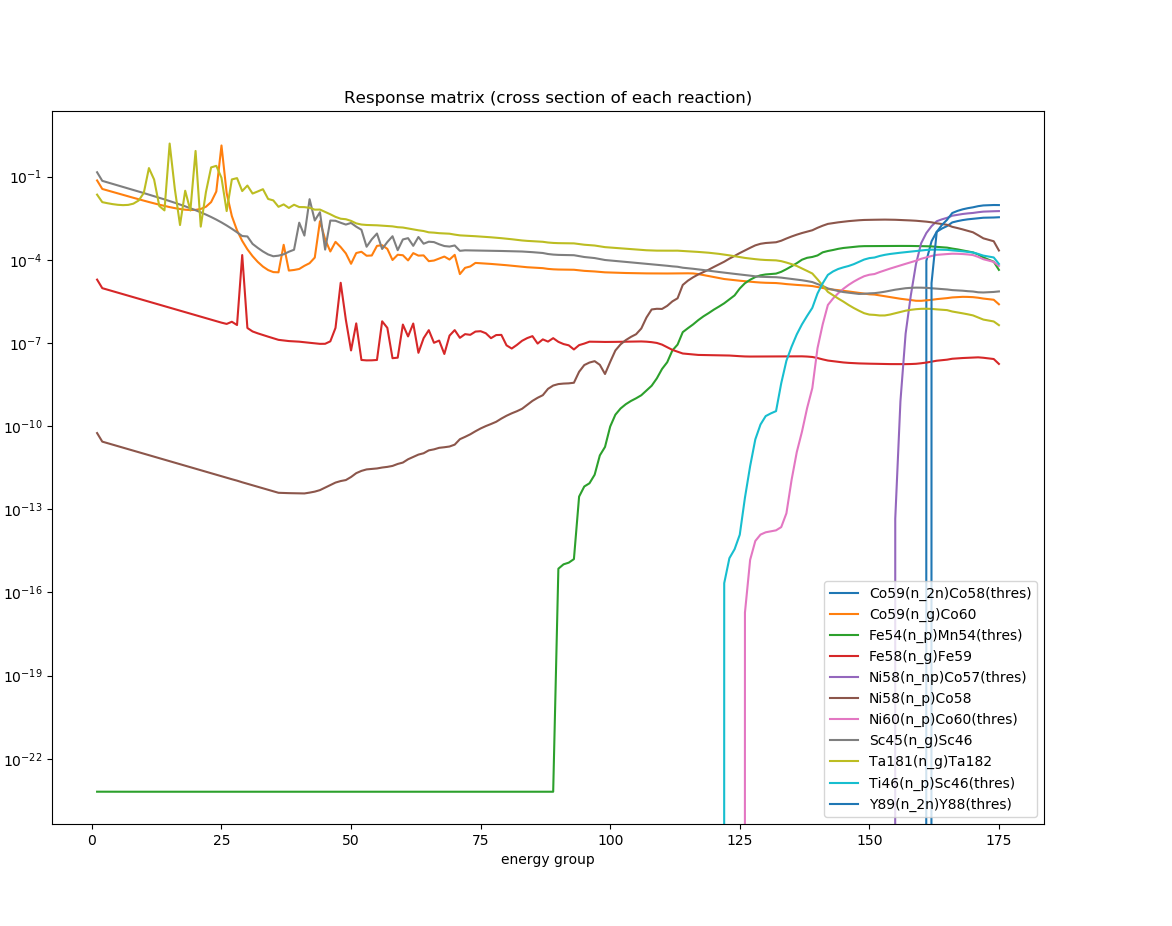
\includegraphics[height=7cm]{PPT/response_matrix.png}
\caption{Microscopic cross-section of each reaction}\label{response_matrix}
These values are obtained from TENDL15 via FISPACT-II \cite{Fispact} at the left edge of each bin in the Vitamin-J group structure. 
\end{figure}
By assuming that the flux per unit lethargy inside each bin are relatively flat (energy independent), the reaction rates contributed by the neutron flux in each bin is then proportional to the product of neutron flux with the microscopic. Symbolically,
\begin{equation} \label{unfolding proportional equation}
    Z_j \propto \sum_i \sigma_{ji} \phi_i
\end{equation}
Akin to the equation \ref{unfolding equation jth component}. Therefore these microscopic cross-section values were used in place of the response function for each of the reaction, assuming the constant of proportionality in equation \ref{unfolding proportional equation} is unity.

\begin{figure}
\centering
\includegraphics[height=5cm]{/home/ocean/Documents/GitHubDir/unfolding/unfolding/unfoldingsuite/neuralnetwork/realoutputEarlyStopping/SelectedNNreplicated/real_fusion_train_spectra.png}
\caption{All fusion spectra used, obtained from \cite{IAEAUKAEACompendium}}\label{RealFusionTrain}
\end{figure}

\subsection{Hyperparameter Optimization}
Since the of each neural network varies according to the hyperparameters used and the data that it is trained on, when investigating the real fusion spectra in section~\ref{RealResults}, multiple neural networks were generated, each with different hyperparameters, to investigate the combination of optimal hyperparameters which may be applied onto this problem.

The following hyperparameters/variables were considered:
\begin{itemize}
    \item activation function used
    \item strategies applied to prevent overfitting
    \begin{itemize}
        \item weight regularization
        \item dropout
    \end{itemize}
    \item number of layers
    \item number of nodes in each layer
    \item number of epochs trained
    \item optimizer algorithm, which has the following parameters:
    \begin{itemize}
        \item momentum term (if applicable)
        \item acceleration term (if applicable)
        \item epsilon (denominator offset parameter) (if applicable)
        \item learning rate
    \end{itemize}
    \item Normalization techniques applied:
    \begin{itemize}
        \item logarithmize the numerical values of features
        % \item take log of labels (spectrum)
        % \item take fourier transform of labels (spectrum)
    \end{itemize}
    \item metric used to evaluate the loss value (See Section \ref{unfolding inverse equation})
    \item Training set/testing set
\end{itemize}
It is nearly impossible to optimize all 14 parameters listed above simulatenously in a grid search as it will be very computationally intensive and laborious. Therefore the following choices were made for each of the hyperparameter to reduce the amount of variations required for the grid search:
\begin{table}[H]
\begin{tabularx}{\textwidth}{lX}
hyperparameter & choice  \\
\hline
activation function & ReLU\cite{ReLU} for nodes in all layers, as it is the most widely used activation fucntion in machine learning and simplest function. \\
overfitting prevention strategies & Early Stopping (stopping the training when the validiation loss does not see improvement in 1000 epochs); while the complexity of the model is restricted by limiting the number of layers to 5 or fewer, so neither dropout or weight regularization will be applied. \\
number of epochs trained & 10000 (subject to change by tensorflow's EarlyStopping callback) \\
\textbf{number of hidden layers} & ranges from 0-5, as this includes all the configurations stated in Table~\ref{NNtopology}. \\
number of nodes in each layer & with refernce to Table~\ref{NNtopology}, the first hidden layer starts with 32 nodes, and logarithmically increases to the last hidden layer, which has 256 nodes. Therefore the six resulting neural network topologies are 11:175, 11:32:175, 11:32:256:175, 11:32:90:256:175, 11:32:64:128:256:175, 11:32:53:90:152:256:175.\\
Optimizer algorithm & using the Adam optimizer\cite{AdamOptimizer} with its default parameters (except for the learning rate, which is specified below), as it is a widely used algorithm in various machine learning projects.\\
\textbf{learning rate} & ranges from $10^{-2}$ to $10^{-2}$, logarithmically spaced, 6 steps per decade.\\
\textbf{metric used to calculate loss value} & ranges from equation \ref{MSE} to \ref{MPSE_including_folded_reaction_rates}\\
\textbf{training set} & Either fusion spectra or fission spectra is used; if fusion spectra is used, then only 80\% (15 spectra) are used as the training set (drawn at random), the remaining 20\%(4) are reserved for testing. \\
testing set & fusion spectra\\
validation set & 20\% of the testing set, drawn at random
\end{tabularx}
\caption{Hyperparameters chosen for building neural networks for investigations}\label{HyperparameterRange}
\end{table}
For combination of variable hyperparameters in Table~\ref{HyperparameterRange} (highlighted with bold typeface), a neural network is created; all other hyperparameters are fixed according to the rows in Table~\ref{HyperparameterRange} with plain font.

\subsection{Results of predicting using the real spectra}
The resulting neural networks were sorted into two groups according to the training set (into "trained on fission" and "trained on fusion"), then each of them were sorted into 4 smaller groups according to the loss value used during training.

For each group of the data, the resulting loss values, MAE, MSE, and std-dev-log(C/E) were all plotted as heatmaps (see Figure~\ref{hyperparametersearchTestLoss} for example).

\begin{figure}
\centering
\includegraphics[width=\linewidth]{/home/ocean/Documents/GitHubDir/unfolding/unfolding/unfoldingsuite/neuralnetwork/realoutputEarlyStopping/SelectedNNreplicated/fusion-fusion/mse_including_folded/fusion-fusion_mse_inc_folded_test_loss.png}
\caption{Heatmap visualizing the loss values of the nerual networks' prediction on the test dataset.}\label{hyperparametersearchTestLoss}
Each square represents a neural network with a particular set of hyperparameters, i.e. learning rate and number of layers. The learning rate increases logarithmically across the x-axis; while the number of layers increase linearly across the y-axis. The number of nodes per layer is increased logarithmically from 32 to 256 (if the number of hidden layers $\ge 2$).\\
Neural networks which performs better has lower loss values, and are represented with darker colours.\\
\end{figure}

General effects of learning rate and number of layers were identified in this manner. For all of the dataset and loss function used concerned, a general trend of increasing testing loss was identified as the number of layers increases; while the learning rate has no significant effect on it (except for causing a periodic oscillation in the testing loss as the learning rate increases logarithmically, which was dismissed as an artefact of the Optimizer algorithm Adam).

However, a closer examination of the performance of these few-layer neural networks reveals that their performance are mediocre. 

For example, below are some of the predicitons made by these few-layer neural networks.

\begin{figure}[H]
\centering
\fluenceandactivities{/home/ocean/Documents/GitHubDir/unfolding/unfolding/unfoldingsuite/neuralnetwork/realoutputEarlyStopping/SelectedNNreplicated/fusion-fusion-final/0927_0215_0_layerfinal_inv_0_test_001_}
\caption{A typical 0-hidden-layer neural network prediction of JET's first wall spectra when trained on fusion spectra (learning rate=0.01)}
\end{figure}

\begin{figure}[H]
\centering
\fluenceandactivities{/home/ocean/Documents/GitHubDir/unfolding/unfolding/unfoldingsuite/neuralnetwork/realoutputEarlyStopping/SelectedNNreplicated/fusion-fusion-final/0927_0217_1_layerfinal_inv_1_test_001_}
\caption{A typical 1-hidden-layer neural network's prediction of JET's first wall spectra when trained on fusion spectra(learning rate=0.01)}
\end{figure}

\begin{figure}
\centering
\fluenceandactivities{/home/ocean/Documents/GitHubDir/unfolding/unfolding/unfoldingsuite/neuralnetwork/realoutputEarlyStopping/SelectedNNreplicated/fusion-fusion/0927_0219_2_layerfinal_inv_2_test_001_}
\caption{A typical 2-hidden-layer neural network prediction of JET's first wall spectra when trained on fusion spectra (learning rate=0.01)}\label{3Layerfusion-fusionJET-FW}
\end{figure}

They are unable to replicate the 14.1 MeV peak at the correct width, and occassionally massively underestimate the high energy tail.

This is likely due to the small dataset of fusion data available. This explanation is supported by the small number of epochs required for training to finish: most of the neural networks finished training in fewer than 50 epochs, i.e. showed no further improvement in the validation loss in the next 1000 epoch after that. This is unusually early stopping of compared to the number of epochs the neural network required to be trained in Section~\ref{Underdetermined case}.

However, one particular extremum showed up on some of the graphs. This is the neural network with the hyperparameters of (learning rate=0.01, topology=11:32:53:90:152:256:175, loss function used = mean-squared-error-including-folded-reaction-rates, eq.~\ref{MSE_including_folded_reaction_rates}), a particularly loss value is obtained. This neural network is found to be as the neural network with the lowest testing loss and testing MSE.

This neural network was able to be reproduce the same results even when its initial weights and biases were initialized using a different tensorflow seed. Therefore its low test loss and test MSE were not coincidencidental, resulting from a numerical instability. It was thought that the neural network was able to generalize from such small dataset, so its predicted spectra were looked into in closer detail.

\begin{figure}[H]
\centering
\fluenceandactivities{/home/ocean/Documents/GitHubDir/unfolding/unfolding/unfoldingsuite/neuralnetwork/realoutputEarlyStopping/SelectedNNreplicated/fusion-fusion/0927_0220_5_layerfinal_inv_5_test_001_}
\caption{JET first wall spectrum as predicted by the optimally performing NN among all NN trained on fusion data.}\label{5Layerfusion-fusionJET-FW}
\end{figure}

But in the end it was concluded that this 5-hidden-layer neural network likely only achieves the above average performance serendipiteously by re-tracing the same average spectrum. This hypothesis is supported by it replicating a very similar spectrum when it attempts to deduce the spectra corresponding to the other two test data.
% Figure~\ref{5Layerfusion-fusionJET-FW} 
% The experiment was repeated using other metrics as the loss values. All four loss value metrics in equation~\ref{MSE} to \ref{MPSE_including_folded_reaction_rates} were tested.

\begin{figure}[H]
\centering
\fluenceandactivities{/home/ocean/Documents/GitHubDir/unfolding/unfolding/unfoldingsuite/neuralnetwork/realoutputEarlyStopping/SelectedNNreplicated/fusion-fusion/0927_0220_5_layerfinal_inv_5_test_002_}
\caption{Water-cooled ceramic breeder blanket TOKAMAK's first wall spectrum as predicted by the optimally performing NN among all NN trained on fusion data.}\label{5Layerfusion-fusionWCCB-FW}
\end{figure}

\begin{figure}[H]
\centering
\fluenceandactivities{/home/ocean/Documents/GitHubDir/unfolding/unfolding/unfoldingsuite/neuralnetwork/realoutputEarlyStopping/SelectedNNreplicated/fusion-fusion/0927_0220_5_layerfinal_inv_5_test_003_}
\caption{Helium-cooled LiPb TOKAMAK's spectrum at the vacuum vessel, as predicted by the optimally performing NN among all NN trained on fusion data.}\label{5Layerfusion-fusionHCLL-VV}
\end{figure}

\begin{figure}[H]
\centering
\fluenceandactivities{/home/ocean/Documents/GitHubDir/unfolding/unfolding/unfoldingsuite/neuralnetwork/realoutputEarlyStopping/SelectedNNreplicated/fusion-fusion/0927_0220_5_layerfinal_inv_5_test_000_}
\caption{Frascati neutron generator spectrum, as predicted by the optimally performing NN among all NN trained on fusion data.}\label{5Layerfusion-fusionFNG}
\end{figure}

% Regardless, we think it might be useful to make it 

% \subsection{potential future improvements}
% 1. In the future we can calculate the spectral index? plug THOSE values in, instead of plugging in the direct values, it might be better at picking out these differences, because it may be more obvious, and can pick it out even when the data is sparse.

\subsection{Benchmarking against existing codes}
\subsubsection{As an unfolding tool}\label{As an unfolding tool}
The method of method of unfolding using neural networks has the inherent advantage of not having to provide an \emph{a priori} spectrum; if sufficient training data (with the correct group structure, and with corresponding reaction rates) has been given to it, a neural network is, theoretically, capable of unfolding any set of new reaction rates into a neutron spectrum. 

Therefore to fairly compare a neural network against the usual unfolding codes, no meaningful information should be given to the unfolding code in form of an \emph{a priori} spectrum. Therefore a naive priori of a flat neutron spectrum (i.e. flux in each bin is simply proportional to the ``size" (lethargy span) of each bin) will be given to the unfolding code before comparing their performance against the neural network unfolded neutron spectra. The unfolding code chosen are GRAVEL and MAXED, as they are the two most commnoly used neutron unfolding code. \cite{LWP_LTIS} \cite{bethColling_TBMD}

% Can be used as the a priori generator?\\
% But it also sucks as an a priori generator, giving , which is only a marginal improvement on the 10.188233 stated in Figure~\ref{gravel_nn_a_priori_JET}
\begin{figure}[H]
\centering
    \fluenceandactivities{/home/ocean/Documents/GitHubDir/unfolding/unfolding/unfoldingsuite/neuralnetwork/realinputEarlyStopping/comparison/real_fusion_test_maxed_test_000_}
    \caption{JET first wall spectrum as unfolded by MAXED upon using a flat neutron spectrum as the \emph{a priori}}\label{maxed_flat_a_priori_JET}
\end{figure}
    
While MAXED performed very poorly (Figure~\ref{maxed_flat_a_priori_JET}) when given a flat \emph{a priori} (giving an MSE value of 53.442406, as defined in equation~\ref{MSE}), GRAVEL was able to unfold a neutron spectrum from the flat \emph{a priori}, though with an underestimated low energy region and overestimated high energy range neutrons.
An MSE value of 10.188233 was obtained when comparing the unfolded spectra against the true spectra in log space. (eq. \ref{MSE})

\begin{figure}
\centering
    \fluenceandactivities{/home/ocean/Documents/GitHubDir/unfolding/unfolding/unfoldingsuite/neuralnetwork/realinputEarlyStopping/comparison/real_fusion_test_gravel_test_001_}
    \caption{JET first wall spectrum as unfolded by GRAVEL upon using a flat neutron spectrum as the \emph{a priori}}\label{gravel_flat_a_priori_JET}
    An average MSE value (as defined in equation\ref{MSE}) of 10.188233 was obtained when comparing the unfolded spectra against the 4 true spectra in testing set.
\end{figure}

While the best performing neural network (Figure~\ref{5Layerfusion-fusionJET-FW}) gives a slightly better result, both Figure~\ref{5Layerfusion-fusionJET-FW} and Figure~\ref{gravel_flat_a_priori_JET} are far from being applicable to real neutron spectrum unfolding, where the unfolding accuracy is much higher (currently the unfolded spectrum gives a total flux that differs from measured total flux by $\pm 7\%$\cite{bethColling_TBMD}). This low accuracy of the solution spectrum is likely due to the small training set of the neural network. This small sample size means that it cannot densely cover the entire domain (feature space) and co-domain (label space) of the fusion neutron spectrum unfolding problem. For the same reason, the neural network's prediction cannot be relied upon for unfolding spectra in new/unknown types of fusion reactor designs, as it has not been shown to extrapolate its predictions with satisfactory performance beyond the very short list of fusion spectra in Appendices~\ref{fission-fusion spectra IAEAUKAEACompendium}.

\subsubsection{As an a priori generator}
When unfolding, an \emph{a priori} spectrum with a reasonably close match to the original spectrum is required as the starting point for an iterative solution search. Given that the neural network did not yield satisfactory unfolding result in the last section, an attempt of using the neural network's output as an \emph{a prior} was made, with the hopes that the neural network's output will be close enough to the true spectrum such that, with further adjustment by the unfolding code such as GRAVEL and MAXED, a reasonable solution spectrum can be reached.

The motivation of using a neural network's output as the \emph{a priori} is that one can save hours of MCNP calculation in order to obtain the response matrix and \emph{a priori} spectrum.

However, this proves to be rather unpromising as well. Even when with best neural network's predictions (Figure~\ref{5Layerfusion-fusionJET-FW}, \ref{5Layerfusion-fusionFNG}, \ref{5Layerfusion-fusionHCLL-VV}, \ref{5Layerfusion-fusionWCCB-FW}), GRAVEL unfolded results that are as poor as when a flat \emph{a priori} was used. An average MSE value of 9.89936 was achieved.
% This is likely because the flux overestimation at the $\le 14.1MeV$ bins leads to a l

And MAXED produced result that are also as meaningless as Figure~\ref{maxed_flat_a_priori_JET}, as the log of the flux in some bins tends to negative infinity.

\begin{figure}
    \centering
    \fluenceandactivities{/home/ocean/Documents/GitHubDir/unfolding/unfolding/unfoldingsuite/neuralnetwork/realinputEarlyStopping/comparison/real_fusion_test_gravel_nn_a_priori_test_001_}
    \caption{JET first wall spectrum as unfolded by GRAVEL upon using the optimal NN's output as the \emph{a priori} spectrum.}\label{gravel_nn_a_priori_JET}
\end{figure}

% \begin{itemize}
%     \item the user doesn't want to commit to hours of MCNP model generation (cite a paper where Lee Packer's group has used a whole MCNP model to get the response matrix and the reaction rates);
%     \item and already has a few similar neutron spectra to pick from;
%     \item want a higher reproducibility/credibility than hand-drawing an a priori with reference to the previous spectra/ averaging over the existing spectra.
% \end{itemize}

\subsection{An attempt at using fission data to predict fusion data}
While fusion spectra are scarce, there is an abundant database of fission neutron spectra. Therefore, it would be ideal if neural networks trained on fission spectra can use it to explain fusion spectra, as we will not run into the issue of not having enough data.

Therefore, the results of the second group of neural networks (trained on fission spectra, tested on fusion spectra) were examined. If there is indeed a transferable underlying pattern that is common to both fission and fusion spectra, e.g. the Maxwellian

But even the best one of them performed very poorly. It uses an MSE loss value equation~\ref{MSE} giving a testing loss of 16.767817. Closer examination of its prediction shows that it is unsuitable for the neutron spectra.

\begin{figure}[H]
\centering
\fluenceandactivities{/home/ocean/Documents/GitHubDir/unfolding/unfolding/unfoldingsuite/neuralnetwork/realoutputEarlyStopping/SelectedNNreplicated/fission-fusion/0927_0226_5_layer_test_mse_1_test_007_}
\caption{(calculated) ITER spectrum as predicted by the optimal NN among all NN trained on fission spectra} \label{fission-fusionBad}
\end{figure}

\begin{figure}[H]
\centering
\fluenceandactivities{/home/ocean/Documents/GitHubDir/unfolding/unfolding/unfoldingsuite/neuralnetwork/realoutputEarlyStopping/SelectedNNreplicated/fission-fusion/0927_0226_5_layer_test_mse_1_test_016_}
\caption{JET first wall spectrum as predicted by the optimal NN among all NN trained on fission spectra}\label{fission-fusionGood}
\end{figure}

(For the record, this neural network (which performed the best out of all neural networks trained on fission spectra) has very similar hyperparameters as the optimally performing neural network identified in the previous section \ref{As an unfolding tool}, differing only in the loss function used. (learning rate = 0.01, topology = 11:32:53:90:152:256:175, loss function used = MSE (eq.\ref{MSE})).)

This suggest that the inverse function required to unfold fission-induced reaction rates in the activation foils is a different inverse function than the inverse function required to unfold the fusion-inducd reaction rates in the activation foils.%In other words, the M-dimensional manifold where fusion spectra exist does not coincide with 

\section{Potential Future improvements}
The techqniue of neural network classification is best applied when the dataset is large, which is not the case with fusion neutron spectra.

In order to improve upon the results observed in this thesis, a much larger dataset, consisting the neutron spectra for magnetic confinement fusion with various plasma and first wall conditions, and potentially of other inertial confinement fusion, should be attained. These data may be obtained by numerical simulations with MCNP, or actual measurements of neutron spectra at various TOKAMAK's and various other fusion facilities; but one has to recognize that neural networks trained on a set of data only creates predictions that are as reliable as its training data.%In other words, if the numerical simulations in MCNP is inaccurate, the neural network will also predict inaccurately.

\begin{itemize}
    \item Use RBF-NN or GRNN, as explained in section~\ref{Literature review}, which are known to perform better under low sample number conditions.
    \item Transfer learning\cite{TransferLearning}: train the neural network with fission data, fix the weights and biases in the half of the neural network, and then train the weights and biases in the remaining half of the neural network using fusion data.
    \item Use Orthogonal Arrays instead of grid searching the entire hyperparameter space, as well as fractional factorial instead of full factorial combinations, as proposed in \cite{RDANNM}, when performing the optimization. This can reduce the amount of time required for the experimentation; or extend the range of hyperparameter space searched in the same amount of time; multiple dimensional space can be search through in the same manner as well. This may reveal a combination of hyperparameter which may lead to a better neural network design for fusion neutron spectra unfolding than the existing optimal design.
\end{itemize}

Lastly, as uncertainty of the neutron spectra needs to be known for the application of fusion neutron measurements, a global sensitivty analysis can be performed on the neural network using a Monte Carlo approach: by repeatedly adding in noise $\delta Z_j$ into the reaction rates $Z_j$ and allowing the neural network to carry out its prediction (forward propagation), the Monte Carlo program will be used to infer the resulting changes $\delta \phi_i$ associated with the neural network's predictions ($\phi_i$), thus propagating uncertainty in the measurements of reaction rates to $\sigma{Z}$ to $\sigma_{\phi}$. An unfolding code suite is already under development in CCFE to allow this to be done systematically.

\section{Conclusion}
A neural network unfolding approach to neutron spectrum unfolding was examined. A grid search for the optimal hyperparameters for the neural network was performed over 4 dimensions (training set used, learning rate, number of layers, and loss function used). The neural network with the best test loss was examined% and scrutinized.

A loss value of 3.?

This is only a slight improvement compared with the loss value of 10.188 obtained when the code was unfolded using GRAVEL.

A loss value of 9. was obtained (MSE in log space, (eq.~\ref{MSE}))

on fission spectra,

\begin{itemize}
    \item What's the loss values
    \item achieved using what topology of NN
    \item trained upon what data
    \item How does it compare to neutron spectrum unfolding using GRAVEL and MAXED
    \item Can we use Fission data to train it? (no)
    \item What's the significance on the unfolding community: should they use it more? Should they improve upon it?
    \item what additional observation did you find regarding training on different dataset.
\end{itemize}

\bibliographystyle{plain}
\bibliography{FACTIUNN}

\begin{appendices}

\section{Neural network building functions tailored for the purpose of neutron spectrum unfolding}
The following contains the class in which the neural network is built.\\
\pythoncode{neuralnetworklibrary.py}{/home/ocean/Documents/GitHubDir/unfolding/unfolding/unfoldingsuite/neuralnetwork/neuralnetworklibrary.py}

\section{Neural network abstractions and controller}
The following contains the higher level abstractions, as well as functions which walks the user through the process of creating a neural network interactively.\\
\pythoncode{neuralnetworktrainer.py}{/home/ocean/Documents/GitHubDir/unfolding/unfolding/unfoldingsuite/neuralnetwork/neuralnetworktrainer.py}

\section{Code for benchmarking}
This code uses 'unfoldingsuite', which contains implementations of MAXED and GRAVEL in python, developed locally at CCFE, to unfold spectra from various a priori. Their performance can then be used as benchmarks for the neural network unfolding results to be compared against.\\
\pythoncode{comparison\_with\_existing.py}{/home/ocean/Documents/GitHubDir/unfolding/unfolding/unfoldingsuite/neuralnetwork/realinputEarlyStopping/comparison/comparison_with_existing.py}

\section{Fully determined simulation data generation}
Creates a 5 energy-bins fluence vector, which is then folded through a 5 $\times$ 5 response matrix; both of which are randomly generated. Each element both were picked from a uniform random distribution larger than 1. The upper bound of the elements in the vector were chosen as 15 and the upper bound of the elements in the response matrix were chosen to be 50.\\
\pythoncode{simple\_non\_singular\_case.py}{/home/ocean/Documents/GitHubDir/unfolding/unfolding/unfoldingsuite/neuralnetwork/demogenerator/simple_non_singular_case.py}

\section{Underdetermined simulation data generation}
For each of the 14 FISPACT reference spectra, each is parametrised into a list of peaks. The height of these peaks were then perturbed to form a `new' spectrum. This `new' spectrum is then folded through a corresponding response matrix.\\
\pythoncode{spectrumrandomizer.py}{/home/ocean/Documents/GitHubDir/unfolding/unfolding/unfoldingsuite/neuralnetwork/demogenerator/spectrumrandomizer.py}

\section{Training and evaluating neural networks on the underdetermined simulation data}
A demonstration of applying neuralnetworktrainer.py on the data generated by spectrumrandomizer.py .\\
\pythoncode{script\_for\_demo.py}{/home/ocean/Documents/GitHubDir/unfolding/unfolding/unfoldingsuite/neuralnetwork/script_for_demo.py}

%IAEA and UKAEA compendium spectra had to be rebinned into the vitamin J spectra in order to be useful.

\section{Selecting from UKAEA and IAEA compendium}
Rebinned spectra from the 212 IAEA + UKAEA compendium \cite{IAEAUKAEACompendium} were sorted into various training and testing sets using the following python program.\\
\pythoncode{getrealdata.py}{/home/ocean/Documents/GitHubDir/unfolding/unfolding/unfoldingsuite/neuralnetwork/Link_UKAEA_IAEA_Compendium/getrealdata.py}

\section{hyperparameter input controller}
Input files for hyperparametertrainer.py using the following code, by iterating through a list of hyperparameters of interest, thus effectively performing a grid search over all hyperparameters.\\
\pythoncode{hyperparameterinput.py}{/home/ocean/Documents/GitHubDir/unfolding/unfolding/unfoldingsuite/neuralnetwork/realinputEarlyStopping/hyperparameterinput.py}
This program can be used to split the into multiple jobs, which can then be submitted to a cluster, parallellizing the process and massively reducing the training and evaluation time of the neural networks. This is done by calling the program with \texttt{python hyperparameterinput.py split}

\section{hyperparameter optimization searching}
List the hyperparameter, training- and testing-sets used to evaluate the neural network on, when the hash\_name of the neural network is given.\\
\pythoncode{hyperparameteroutput.py}{/home/ocean/Documents/GitHubDir/unfolding/unfolding/unfoldingsuite/neuralnetwork/realoutputEarlyStopping/hyperparameteroutput.py}

\section{Loss value visualizer}
When given the names of the training- and testing-set, the following code show the loss values (and other metrics) of the neural networks with different hyperparameters achieved on them. This is plotted as a heat map, over the two dimensions of hyperparameters varied, which are `number of layers' (y-axis) and `learning rate' (x-axis) respectively.\\
\pythoncode{hyperparameteroptimizer.py}{/home/ocean/Documents/GitHubDir/unfolding/unfolding/unfoldingsuite/neuralnetwork/realoutputEarlyStopping/hyperparameteroptimizer.py}

\section{Parametrisation of the FISPACT reference spectra}
\begin{table}[H]
\begin{tabular}{ccccccc}
distribution&$\mu$&$\sigma$&A&$\mu_{corr}$&$\sigma_{corr}$&$A_{corr}$\\
\hline
log-normal&-1.48e+01&1.20e+00&1.00e+00&1.0&0.6536070787201796&0.6465171468399362\\
log-normal&-1.17e+01&1.20e+00&5.54e+01&1.0&0.6923014193474084&0.41834840464375106\\
log-normal&-8.61e+00&1.20e+00&3.07e+03&1.0&0.5802541895436414&0.3391941243798774\\
log-normal&-5.52e+00&1.20e+00&1.70e+05&1.0&0.769982827091882&0.5451675762326162\\
log-normal&-2.43e+00&1.20e+00&9.40e+06&1.0&0.6705439760036781&0.6056530392573959\\
log-normal&6.55e-01&1.20e+00&5.20e+08&1.0&0.6485812808091918&0.6213932412543168\\
log-normal&3.74e+00&1.20e+00&2.88e+10&1.0&0.33687762989691133&1.754564218248171\\
\hline
log-normal&-1.44e+01&1.50e+00&1.00e+09&1.0&1.1087020488776023&1.2837241483881578\\
log-normal&-8.60e+00&1.50e+00&3.22e+11&1.0&0.7012835343191862&0.6774642293787084\\
log-normal&-2.83e+00&1.50e+00&1.04e+14&1.0&0.9732542967472964&1.0011605034609532\\
log-normal&2.94e+00&1.50e+00&3.33e+16&1.0&0.9872173030484698&0.99379684387792\\
normal&1.41e+01&4.00e-01&1.00e+19&1.023&1.0500657332932959&1.128662095083972\\
\hline
log-normal&-1.54e+01&1.10e+00&1.00e+03&1.0&1.0295086712444834&1.0871973190897086\\
log-normal&-1.18e+01&1.10e+00&3.59e+04&1.0&1.0470576309590907&1.1133327728488918\\
log-normal&-8.26e+00&1.10e+00&1.29e+06&1.0&0.9512570373593815&1.0428424889188541\\
log-normal&-4.67e+00&1.10e+00&4.64e+07&1.0&1.1561895212201019&1.1532829852822521\\
log-normal&-1.09e+00&1.10e+00&1.67e+09&1.0&1.0181223850843093&1.018626898626218\\
normal&1.41e+01&4.00e-01&1.00e+10&1.0&1.32722437503459&1.8671520930196117\\
normal&2.45e+00&1.00e-01&1.00e+12&1.0&0.8152984470618088&0.5530754449242801\\
\hline
log-normal&-1.26e+01&2.00e+00&1.00e+05&1.0&1.094149298940297&1.17454890924765\\
log-normal&-7.12e+00&2.00e+00&2.47e+07&1.0&1.7120265659905378&1.12525321665773\\
log-normal&-1.61e+00&2.00e+00&6.08e+09&1.0&1.2209065015914118&1.5577920026942778\\
log-normal&3.89e+00&2.00e+00&1.50e+12&1.0&1.0538009149767102&1.5525710802981993\\
normal&1.41e+01&4.00e-01&1.00e+14&1.0&0.9946385566258605&1.1958058458498946\\
\hline
log-normal&3.00e+00&2.00e+00&1.00e+13&1.0&0.985831182477408&1.191099325784018\\
log-normal&-3.20e+00&2.00e+00&1.00e+11&1.0&1.0163826189572225&1.037504496747917\\
normal&1.41e+01&4.00e-01&1.00e+14&1.0&1.132214159680078&1.3221159758391146\\
\hline
log-normal&-5.60e+00&2.30e+00&4.00e+05&1.0&0.912896343655827&0.9707283164160951\\
log-normal&-4.80e+00&5.00e-01&1.00e+06&1.0&0.9724734344690737&1.3093741751167056\\
log-normal&3.00e+00&1.80e+00&5.00e+09&1.0&1.1626572027366295&0.8373153796607655\\
normal&1.41e+01&4.00e-01&1.00e+10&1.0&1.1868044101095476&1.555176012813058\\
\hline
normal&1.35e+01&2.00e+00&2.00e+20&1.0&1.0094598165344801&1.0398929376955228\\
log-normal&-2.40e+00&3.50e-01&1.00e+14&1.0&0.9999755394847119&1.0437028488962274\\
log-normal&-1.43e+00&3.50e-01&5.54e+14&1.0&1.0040524756949494&1.2576232255047286\\
log-normal&-4.47e-01&3.50e-01&3.07e+15&1.0&1.0213050801706227&1.2668031933646988\\
log-normal&5.31e-01&3.50e-01&1.70e+16&1.0&1.0185780833110203&1.3543132306863206\\
log-normal&1.51e+00&3.50e-01&9.40e+16&1.0&1.0622261078184665&1.1481233202529897
\end{tabular}
\caption{In descending order: each section represents the parameters used to parametrise the spectra of: JAEA-FNS, Frascati-NG, ITER-DD, ITER-DT, DEMO-HCPB-FW, JET-FW, NIF-Ignition. The 2-4${}^{th}$ columns indicate the guess value inputted, while the last 3 columns indicate the correction factor multiplied onto them. E.g. $\mu_{final} = \mu * \mu_{corr}$}\label{ParametrisationParameters}
\end{table}
\section{neutron spectra extraed from the IAEA + UKAEA compendium}\label{fission-fusion spectra IAEUKAEACompendium}
List of all fission data
\begin{longtable}{llll}[H]
title & type &Measured/Calculated\\
\hline
PR\_PWR\_CZECH\_6 & PR & Czech PWR, circ. pumps, near cold side, p2  & M\\
PR\_BWR\_DUNG\_1 & PR & BWR, Dungeness, boiler cell  & M\\
RFT\_PU\_3 & RFT & Pu reprocessing plant, fuel pin assembly  & M\\
RFT\_MOX\_4 & RFT & Fresh MOX, borated water shield  & M\\
PR\_GCR\_1 & PR & CH1 GC reactor  & M\\
RFT\_PU\_2 & RFT & Pu reprocessing plant, well shielded  & M\\
PR\_PWR\_CZECH\_2 & PR & Czech PWR, check room, under reactor, p5  & M\\
PR\_BWR\_SW\_4 & PR & BWR (Switzerland), under access  & M\\
PR\_GCR\_3 & PR & Trawsfynydd GC reactor, position S3  & M\\
PR\_PWR\_CZECH\_4 & PR & Czech PWR, check room, under reactor, p13  & M\\
PR\_BWR\_SW\_13 & PR & PWR (Switzerland), behind generator  & M\\
UKAEA\_029\_EBR-2 & UKAEA\_PR & EBR-2 spectra in 29 energy groups & M\\
PR\_BWR\_SW\_8 & PR & BWR (Switzerland), near lock, closed  & M\\
PR\_PWR\_CZECH\_7 & PR & Czech PWR, circ. pumps, hot side, p3  & M\\
PR\_BWR\_SW\_16 & PR & PWR (Switzerland), 33 cm behind door  & M\\
UKAEA\_1102\_BWR-MOX-Gd-0 & UKAEA\_PR & BWR-MOX-Gd-0 spectra in 1102 energy groups & M\\
UKAEA\_100\_HFIR-lowres & UKAEA\_PR & HFIR-lowres spectra in 100 energy groups & M\\
UKAEA\_1102\_PWR-MOX-15 & UKAEA\_PR & PWR-MOX-15 spectra in 1102 energy groups & M\\
BT\_FRM\_2 & BT & FRM II beam, unfiltered  & M\\
RFT\_PU\_1 & RFT & Pu reprocessing plant, little shielding, location 1  & M\\
PR\_BWR\_SW\_14 & PR & PWR (Switzerland), at reactor axis  & M\\
PR\_PWR\_WOLFCREEK\_3 & PR & PWR, Wolf Creek, power 50\%, 2026¢ level by valves  & M\\
RFT\_PU\_USA\_4 & RFT & TRU plant, at conduit exit, less shielding  & M\\
PR\_PWR\_CZECH\_13 & PR & Czech PWR, reactor hall, near cap, p10  & M\\
IS\_TRU\_6 & IS & TRU plant, 25 g AmO2 in container  & M\\
PR\_BWR\_SW\_2 & PR & BWR (Switzerland), at bend of maze  & M\\
PR\_BWR\_CAORSO\_8 & PR & BWR, Caorso, position 4  & C\\
PR\_PWR\_WOLFCREEK\_1 & PR & PWR, Wolf Creek, power 50\%, at PH 2047¢ level  & M\\
UKAEA\_1102\_PWR-UO2-Gd-15 & UKAEA\_PR & PWR-UO2-Gd-15 spectra in 1102 energy groups & M\\
PR\_BWR\_DUNG\_3 & PR & BWR, Dungeness, on the walkway  & M\\
PR\_BWR\_CAORSO\_3 & PR & BWR, Caorso, position 3  & M\\
PR\_BWR\_SW\_5 & PR & BWR (Switzerland), at stairwell  & M\\
BT\_LVR15\_1 & BT & LVR-15, epithermal beam  & C\\
UKAEA\_1102\_BWR-MOX-Gd-15 & UKAEA\_PR & BWR-MOX-Gd-15 spectra in 1102 energy groups & M\\
PR\_PWR\_CZECH\_10 & PR & Czech PWR, reactor hall, at cap, p7  & M\\
IS\_TRU\_9 & IS & 25 Ci Am ceramics, no shield  & M\\
RFT\_WWER\_CASK\_3 & RFT & Transport cask C30/KB54, in corridor at 45 cm  & M\\
RFT\_WWER\_CASK\_1 & RFT & Transport cask C30/KB54, in a hall at 45 cm  & M\\
PR\_GCR\_2 & PR & CH2 GC reactor  & M\\
BT\_BMRR\_1 & BT & BMRR spectra, filtered by 34 cm Al/AlF3  & M\\
UKAEA\_172\_Phenix & UKAEA\_PR & Phenix spectra in 172 energy groups & M\\
PR\_TRAWS\_1 & PR & Trawsfynnydd, filter gallery  & M\\
RFT\_TN12\_1 & RFT & TN-12 fuel container at Valognes  & M\\
RFT\_PU\_USA\_1 & RFT & TRU plant, lightly shielded glovebox 1  & M\\
RFT\_VALDUC\_1 & RFT & Pu reprocessing at Valduc  & M\\
RFT\_PU\_USA\_2 & RFT & TRU plant, heavily shielded glovebox 1  & M\\
PR\_HINKLEY\_2 & PR & Hinkley Point, filter gallery  & M\\
BT\_ACCEPI\_1 & BT & Accelerator based epithermal beam  & M\\
PR\_RINGHALS\_3 & PR & Ringhals, point P  & M\\
UKAEA\_616\_HFR-high & UKAEA\_PR & HFR-high spectra in 616 energy groups & M\\
PR\_BWR\_SW\_15 & PR & PWR (Switzerland), 40 cm behind door  & M\\
PR\_BWR\_CAORSO\_4 & PR & BWR, Caorso, position 4  & M\\
PR\_BWR\_SW\_6 & PR & BWR (Switzerland), 16 m level, near pump  & M\\
BT\_BMRR\_1\_1 & BT & BMRR beam  & M\\
PR\_BWR\_SW\_10 & PR & PWR (Switzerland), in front of containment  & M\\
PR\_BWR\_CAORSO\_7 & PR & BWR, Caorso, position 3  & C\\
RFT\_MOX\_2 & RFT & MOX transport cask, ver. 03  & M\\
UKAEA\_198\_PWR-RPV & UKAEA\_PR & PWR-RPV spectra in 198 energy groups & M\\
UKAEA\_407\_Bigten & UKAEA\_FIS & Bigten spectra in 407 energy groups & M\\
UKAEA\_1102\_BWR-UO2-Gd-40 & UKAEA\_PR & BWR-UO2-Gd-40 spectra in 1102 energy groups & M\\
BT\_BMRR\_2 & BT & BMRR spectra, filtered by 22 cm 7LiF  & M\\
UKAEA\_1102\_PWR-UO2-15 & UKAEA\_PR & PWR-UO2-15 spectra in 1102 energy groups & M\\
BT\_BMRR\_3 & BT & BMRR spectra, filtered by 17 cm D2O  & M\\
RFT\_1393\_2 & RFT & Transport cask 1393(2)  & M\\
BT\_BNCT\_PETTEN\_1 & BT & BNCT in Petten, HB11 filtered beam  & M\\
BT\_FRM\_3 & BT & FRM II beam, filtered  & M\\
UKAEA\_1102\_BWR-UO2-Gd-15 & UKAEA\_PR & BWR-UO2-Gd-15 spectra in 1102 energy groups & M\\
PR\_PWR\_GOSGEN\_1 & PR & PWR, Gosgen, position 1  & M\\
UKAEA\_198\_BWR-RPV & UKAEA\_PR & BWR-RPV spectra in 198 energy groups & M\\
RFT\_PU\_USA\_5 & RFT & TRU plant, lightly shielded glovebox 2  & M\\
PR\_RINGHALS\_4 & PR & Ringhals, point B2  & M\\
IS\_TRU\_7 & IS & TRU plant, 244Cm in glovebox, no shield  & M\\
PR\_BWR\_CAORSO\_2 & PR & BWR, Caorso, position 2  & M\\
RFT\_PU\_USA\_3 & RFT & TRU plant, at operator desk  & M\\
UKAEA\_1102\_PWR-UO2-0 & UKAEA\_PR & PWR-UO2-0 spectra in 1102 energy groups & M\\
PR\_RINGHALS\_5 & PR & Ringhals, point B4  & M\\
PR\_BWR\_CAORSO\_5 & PR & BWR, Caorso, position 1  & C\\
PR\_PWR\_WOLFCREEK\_2 & PR & PWR, Wolf Creek, power 50\%, 2 m from PH 2047¢ level  & M\\
PR\_RINGHALS\_1 & PR & Ringhals, point D  & M\\
PR\_BWR\_CAORSO\_6 & PR & BWR, Caorso, position 2  & C\\
PR\_BWR\_SW\_7 & PR & BWR (Switzerland), 16 m level, near tap  & M\\
UKAEA\_172\_Paluel & UKAEA\_PR & Paluel spectra in 172 energy groups & M\\
RFT\_POLLUX\_2 & RFT & Pollux container above ground level  & M\\
PR\_BWR\_CAORSO\_1 & PR & BWR, Caorso, position 1  & M\\
PR\_PWR\_CP\_1 & PR & CP reactor, site 5, SPUNIT code  & M\\
PR\_PWR\_CZECH\_8 & PR & Czech PWR, circ. pumps, near door, p4  & M\\
PR\_BWR\_SW\_9 & PR & BWR (Switzerland), near lock, open  & M\\
RFT\_MOX\_1 & RFT & MOX transport cask, ver. 02  & M\\
PR\_PWR\_CP\_2 & PR & CP reactor, site 6, SPUNIT code  & M\\
PR\_PWR\_CZECH\_3 & PR & Czech PWR, check room, in middle, p12  & M\\
RFT\_WWER\_CASK\_4 & RFT & Transport cask C30/KB54, in corridor at 2 m  & M\\
PR\_PWR\_CZECH\_11 & PR & Czech PWR, reactor hall, at valve, p8  & M\\
IS\_TRU\_8 & IS & Am–Be sources in gloveboxes in line  & M\\
PR\_BWR\_SW\_11 & PR & PWR (Switzerland), 1 m from platform  & M\\
UKAEA\_070\_Cf252 & UKAEA\_IS & Cf252 spectra in 70 energy groups & M\\
UKAEA\_1102\_PWR-MOX-40 & UKAEA\_PR & PWR-MOX-40 spectra in 1102 energy groups & M\\
PR\_PWR\_CZECH\_12 & PR & Czech PWR, reactor hall, at generator, p9  & M\\
UKAEA\_1102\_PWR-MOX-0 & UKAEA\_PR & PWR-MOX-0 spectra in 1102 energy groups & M\\
PR\_HINKLEY\_1 & PR & Hinkley Point, pile cap  & M\\
BT\_ACC\_2 & BT & Gantry spectrum  & C\\
PR\_PWR\_WOLFCREEK\_4 & PR & PWR, Wolf Creek, power 100\%, at PH 2047¢ level  & M\\
PR\_PWR\_CZECH\_9 & PR & "Czech PWR, circ. pumps, 4 \& 4, p11 " & M\\
PR\_BWR\_SW\_3 & PR & BWR (Switzerland), at drywell  & M\\
UKAEA\_1102\_BWR-UO2-Gd-0 & UKAEA\_PR & BWR-UO2-Gd-0 spectra in 1102 energy groups & M\\
BT\_ACC\_1 & BT & Accelerator based spectrum, 2.5 MeV protons on 7Li  & C\\
RFT\_POLLUX\_1 & RFT & Pollux container in salt mine  & M\\
RFT\_LK100\_1 & RFT & LK-100 fuel container at La Hague, position1  & M\\
UKAEA\_616\_HFR-low & UKAEA\_PR & HFR-low spectra in 616 energy groups & M\\
RFT\_MOX\_5 & RFT & Fresh MOX, no shield  & M\\
RFT\_NTL\_1 & RFT & Transport cask NTL-111, at 115 cm  & M\\
RFT\_HANAU\_1 & RFT & Fission material deposition, BS measurements  & M\\
PR\_PWR\_WOLFCREEK\_5 & PR & PWR, Wolf Creek, power 100\%, 2026¢ level at loop penetration  & M\\
UKAEA\_172\_Superphenix & UKAEA\_PR & Superphenix spectra in 172 energy groups & M\\
RFT\_WWER\_CASK\_2 & RFT & Transport cask C30/KB54, in a hall at 2 m  & M\\
RFT\_MOX\_3 & RFT & New MOX at 20 cm, no shield  & M\\
PR\_PWR\_CZECH\_5 & PR & Czech PWR, check room, corridor, p6  & M\\
PR\_PWR\_CP\_4 & PR & CP reactor, site 4, YOGI code  & M\\
RFT\_HANAU\_2 & RFT & Fission material deposition, LS measurements  & M\\
UKAEA\_1102\_PWR-UO2-40 & UKAEA\_PR & PWR-UO2-40 spectra in 1102 energy groups & M\\
PR\_GCR\_4 & PR & Trawsfynydd GC reactor, position S4  & M\\
UKAEA\_1102\_PWR-UO2-Gd-40 & UKAEA\_PR & PWR-UO2-Gd-40 spectra in 1102 energy groups & M\\
PR\_RINGHALS\_2 & PR & Ringhals, point E  & M\\
BT\_SPALL\_1 & BT & Spallation source, 72 MeV protons on W  & C\\
RFT\_LK100\_2 & RFT & LK-100 fuel container at La Hague, position 2  & M\\
PR\_BWR\_SW\_12 & PR & PWR (Switzerland), 3 m from platform  & M\\
PR\_PWR\_GOSGEN\_2 & PR & PWR, Gosgen, position 2  & M\\
UKAEA\_1102\_PWR-UO2-Gd-0 & UKAEA\_PR & PWR-UO2-Gd-0 spectra in 1102 energy groups & M\\
RFT\_PU\_5 & RFT & Pu reprocessing plant, little shielding, location 5  & M\\
RFT\_NTL\_2 & RFT & Transport cask NTL-111, at 367 cm  & M\\
RFT\_PU\_4 & RFT & Pu reprocessing plant, little shielding, location 4  & M\\
PR\_PWR\_CP\_3 & PR & CP reactor, site 4, SPUNIT code  & M\\
PR\_PWR\_CZECH\_1 & PR & Czech PWR, circ. pumps, cold side, p1  & M\\
PR\_BWR\_DUNG\_2 & PR & BWR, Dungeness, on the roof  & M\\
BT\_FRM\_1 & BT & FRM I beam  & M\\
RFT\_1392\_1 & RFT & Transport cask 1392(1)  & M\\
UKAEA\_1102\_BWR-MOX-Gd-40 & UKAEA\_PR & BWR-MOX-Gd-40 spectra in 1102 energy groups & M\\
PR\_BWR\_SW\_1 & PR & BWR (Switzerland), at maze entrance  & M
% \caption{}
\end{longtable}

List of all fusion data used as the training set
\begin{longtable}{llll}[H]
title&type&description&Measured/Calculated\\
\hline
UKAEA\_616\_DEMO-HCPB-VV&UKAEA\_FUS&DEMO-HCPB-VV spectra in 616 energy groups&M\\
UKAEA\_150\_NIF-ignition&UKAEA\_FUS&NIF-ignition spectra in 150 energy groups&M\\
UKAEA\_616\_DEMO-HCPB-BP&UKAEA\_FUS&DEMO-HCPB-BP spectra in 616 energy groups&M\\
UKAEA\_616\_WCLL-VV&UKAEA\_FUS&WCLL-VV spectra in 616 energy groups&M\\
UKAEA\_616\_HCPB-VV&UKAEA\_FUS&HCPB-VV spectra in 616 energy groups&M\\
UKAEA\_616\_WCCB-VV&UKAEA\_FUS&WCCB-VV spectra in 616 energy groups&M\\
UKAEA\_175\_JAEA-FNS&UKAEA\_FUS&JAEA-FNS spectra in 175 energy groups&M\\
UKAEA\_175\_ITER-DD&UKAEA\_FUS&ITER-DD spectra in 175 energy groups&M\\
UKAEA\_161\_LMJ-g&UKAEA\_FUS&LMJ-g spectra in 161 energy groups&M\\
UKAEA\_175\_ITER-DT&UKAEA\_FUS&ITER-DT spectra in 175 energy groups&M\\
UKAEA\_616\_HCPB-FW&UKAEA\_FUS&HCPB-FW spectra in 616 energy groups&M\\
UKAEA\_616\_DEMO-HCPB-FW&UKAEA\_FUS&DEMO-HCPB-FW spectra in 616 energy groups&M\\
UKAEA\_175\_TUD-NG&UKAEA\_FUS&TUD-NG spectra in 175 energy groups&M\\
UKAEA\_616\_WCLL-FW&UKAEA\_FUS&WCLL-FW spectra in 616 energy groups&M\\
UKAEA\_616\_HCLL-FW&UKAEA\_FUS&HCLL-FW spectra in 616 energy groups&M
\end{longtable}

List of all fusion data used as the testing set
\begin{longtable}{llll}[H]
title&type&description&Measured/Calculated\\
\hline
UKAEA\_175\_Frascati-NG&UKAEA\_FUS&Frascati-NG spectra in 175 energy groups&M\\
UKAEA\_100\_JET-FW&UKAEA\_FUS&JET-FW spectra in 100 energy groups&M\\
UKAEA\_616\_WCCB-FW&UKAEA\_FUS&WCCB-FW spectra in 616 energy groups&M\\
UKAEA\_616\_HCLL-VV&UKAEA\_FUS&HCLL-VV spectra in 616 energy groups&M
\end{longtable}

\end{appendices}

\end{document}

% With data augmentation: it works quite well, even when there are only 2 layers.
%WIthout data augmentation: Suffer from a big problem of insufficient data.
%`